\documentclass[a4paper, 12pt, oneside, BCOR1cm, toc=chapterentrywithdots]{scrbook}

% --- Encoding and Fonts ---
\usepackage[utf8]{inputenc}
\usepackage[T1]{fontenc}
\usepackage{pifont}
\usepackage{lmodern} % Optional, better default font

% --- Common Packages ---
\usepackage{graphicx}
\usepackage{makeidx}
\usepackage[colorlinks=false]{hyperref}
\usepackage{tocbibind}
\usepackage{blindtext}
\usepackage{subfigure} 
\usepackage{acronym}
\usepackage{multicol}
\KOMAoptions{parskip=half}

\usepackage{tikz}
\usepackage{tabularx}
\usepackage{array}
\usepackage{makecell}

\usepackage{graphicx} % for \resizebox
\usepackage{tikz}
\usetikzlibrary{arrows.meta,positioning,fit,backgrounds}

\renewcommand{\arraystretch}{1.4}
\newcommand{\cmark}{\ding{51}} % check mark
\newcommand{\xmark}{\ding{55}} % cross mark
\usepackage[numbers]{natbib}

\setcounter{secnumdepth}{3}


% --- Hyperref Setup ---
\hypersetup{
  bookmarksnumbered=true,
  hyperindex=true,
  bookmarksopen=true,
  bookmarksopenlevel=1,
  pdfborder=0 0 0
}

% --- Custom Star Symbols ---
\newcommand{\starfull}{\ding{72}}   % Full star
\newcommand{\starhalf}{\ding{73}}   % Half star
\newcommand{\starzero}{\ding{78}}   % Empty star

% --- TOC Appearance Fixes ---
\renewcommand*{\tableofcontents}{%
  \begingroup
  \tocsection
  \tocfile{\contentsname}{toc}
  \endgroup
}
\renewcommand*{\listoffigures}{%
  \begingroup
  \tocsection
  \tocfile{\listfigurename}{lof}
  \endgroup
}
\renewcommand{\listoftables}{
  \begingroup
  \tocsection
  \tocfile{\listtablename}{lot}
  \endgroup
}

\makeindex

\begin{document}

% =====================================================
% FRONTMATTER: Roman numeral page numbering
% =====================================================
\frontmatter

% -------- Title Page --------
\begin{titlepage}
  {
    \begin{center}
        \raisebox{-1ex}{\includegraphics[scale=1.4]{images/TU_Chemnitz_positiv_gruen.pdf}}\\
    \end{center}
    \vspace{0.5cm}
  }
  \begin{center}
    \LARGE{\textbf{ulti-Agent Template Filling using LLMs: Design and Comparative Evaluation with Speech Input Case Study}}\\
    \vspace{1cm}
    \Large{\textbf{Master Thesis}}\\ 
    \vspace{0.5cm}
    Submitted in Fulfilment of the\\
    Requirements for the Academic Degree\\
    M.Sc. Web Engineering\\
    \vspace{0.5cm}
    Dept. of Computer Science\\
    Chair of Computer Engineering
  \end{center}
  \vspace{1cm}
  Submitted by: Huzefa Ismail Jadliwala\\
  Student ID: 806286\\
  Date: 07.07.2025\\
  \vspace{0.3cm}\\
  Internal Supervising tutor: Verena Traubinger \\
  External Supervising tutor: Dr. Christoph Carl Kling \\
\end{titlepage}

% -------- Abstract --------
\addchap*{Abstract}
\addcontentsline{toc}{chapter}{Abstract}
This thesis presents a modular, multi-agent system for converting unstructured spoken language into structured templates using large language models (LLMs). The focus is on real-world domains such as healthcare, manufacturing, and administration. Traditional monolithic LLM approaches often struggle with ambiguous or noisy inputs, lack adaptability, and provide limited transparency. To address these limitations, the proposed Invox system decomposes the task into four subtasks—transcription interpretation, field mapping, value inference, and result verification—handled by specialized LLM agents. Five architectural strategies are implemented and compared: Single-Pass Full Input, Iterative Single-Field Processing, Multi-LLM Consensus (Full), Multi-LLM Consensus (Iterative), and Hybrid Refinement. The system integrates tools such as Whisper, GPT-4, Claude, and DeepSeek, and is evaluated across benchmarks including the MUC-4 dataset and a real-world industrial corpus from steel manufacturing. The evaluation focuses on accuracy, consistency, latency, cost-efficiency, and modularity, offering insight into the trade-offs and design choices involved in deploying agent-based LLM architectures for speech-driven template filling.

\textbf{Keywords: Large Language Models (LLMs), Multi-Agent Systems, Template Filling, Prompt Engineering, Natural Language Understanding, Speech-to-Text Processing}

% -------- Acknowledgment --------
\chapter*{Acknowledgment}
\addcontentsline{toc}{chapter}{Acknowledgment}
I would like to express my deepest gratitude to all those who supported and guided me throughout the development of this Master's thesis.

First and foremost, I am sincerely thankful to my internal supervising tutor, Verena Traubinger, for her dedicated support, timely feedback, and constructive suggestions throughout the entire process. Her patience, encouragement, and willingness to engage in critical discussions greatly contributed to both the conceptual and practical aspects of my work.

I would also like to extend my heartfelt appreciation to my external supervising tutor, Dr. Christoph Carl Kling, for his expert guidance and valuable insights. His technical knowledge and practical experience provided a crucial perspective that helped refine and strengthen the foundation of this thesis. His continuous motivation and thoughtful remarks challenged me to think critically and aim for a high-quality outcome.

Furthermore, I would like to thank the faculty members and academic staff of the program for creating an intellectually stimulating environment that inspired me to pursue research in this domain.

Special thanks also go to my friends and colleagues for their encouragement, helpful discussions, and emotional support during challenging times. I am especially grateful to my family for their unwavering belief in me, their unconditional support, and their motivation throughout my academic journey.

This thesis would not have been possible without the contributions and support of all these individuals. To each of them, I extend my sincere thanks.


% -------- Task Description --------
\chapter*{Task Description}
\addcontentsline{toc}{chapter}{Task Description}
In domains such as healthcare, manufacturing, and administration, converting unstructured spoken language into structured forms is a critical yet challenging task. Traditional approaches using large language models (LLMs) typically employ monolithic systems that attempt to complete the entire template filling process in a single step. While computationally efficient, these systems are often brittle: they struggle with incomplete or ambiguous inputs, lack modularity for domain adaptation, and provide limited transparency when dealing with domain-specific terminology, noisy transcriptions, or real-world operational conditions.


This thesis proposes a modular, multi-agent approach to template filling, implemented through the \textbf{Invox} system. Instead of treating the problem as a single LLM task, Invox decomposes it into subtasks—transcription interpretation, field mapping, value inference, and result verification—each handled by dedicated LLM agents. The system leverages state-of-the-art components such as Whisper for transcription, GPT-4 and Claude for reasoning, and DeepSeek for semantic validation. Five architectural strategies are explored: (1) Single-Pass Full Input, (2) Iterative Single-Field Processing, (3) Multi-LLM Consensus (Full), (4) Multi-LLM Consensus (Iterative), and (5) Hybrid Refinement. These differ in terms of prompt structure, processing granularity, and verification mechanisms. All approaches are evaluated using the same criteria: accuracy, consistency, latency, cost-efficiency, and modularity. Datasets include the benchmark MUC-4 corpus and a real-world industrial dataset from steel manufacturing shift reports. The goal is not only to assess individual method performance, but to better understand the trade-offs introduced by modular, agent-based LLM systems in real-world deployment contexts.


The objective of this thesis is the creation of a solution or the combination of existing approaches to solve the problem described above of filling out templates with the help of Large Language Models. This comprises the following parts. An analysis of the state of the art on LLMs and prompt engineering, multi-agent systems, tools for filling out templates, and other relevant work. The thesis includes the implementation and comparison of five different approaches for a solution. A suitable evaluation should be conducted, where the approaches are tested on datasets regarding a set of benchmarks and the elicited requirements based on the literature research.


% -------- TOC, List of Figures, Tables --------
\tableofcontents
\listoffigures
\listoftables

% -------- List of Abbreviations --------
\chapter*{List of Abbreviations}
\addcontentsline{toc}{chapter}{List of Abbreviations}
\begin{multicols}{2}
\begin{acronym}[Whisper] % Longest acronym for spacing

% === Core System Components ===
\acro{STT}{Speech-to-Text}\label{acro:STT}
\acro{RAG}{Retrieval-Augmented Generation}\label{acro:RAG}
\acro{IE}{Information Extraction}\label{acro:IE}
\acro{CF}{Consistency Formatting}\label{acro:CF}
\acro{VER}{Verification}\label{acro:VER}

% === Strategy Identifiers ===
\acro{S1}{Strategy 1: Single-Pass Full Input}\label{acro:S1}
\acro{S2}{Strategy 2: Iterative Single-Field}\label{acro:S2}
\acro{S3}{Strategy 3: Multi-LLM Consensus (Full)}\label{acro:S3}
\acro{S4}{Strategy 4: Multi-LLM Per-Field}\label{acro:S4}
\acro{S5}{Strategy 5: LangExtract Baseline}\label{acro:S5}

% === Requirements ===
\acro{R1}{Requirement 1: Consistency}\label{acro:R1}
\acro{R2}{Requirement 2: Information Extraction}\label{acro:R2}
\acro{R3}{Requirement 3: Transparency}\label{acro:R3}
\acro{R4}{Requirement 4: User Correction}\label{acro:R4}
\acro{R5}{Requirement 5: Learning and Adaptation}\label{acro:R5}
\acro{R6}{Requirement 6: Usability}\label{acro:R6}

% === Evaluation Metrics ===
\acro{OBS}{Overall Baseline Score}\label{acro:OBS}
\acro{NES}{Nonempty Score}\label{acro:NES}
\acro{EAI}{Empty Advantage Index}\label{acro:EAI}
\acro{SF1}{Soft F1 Score}\label{acro:SF1}
\acro{FDA}{Fill-Decision Accuracy}\label{acro:FDA}
\acro{HR}{Hallucination Rate}\label{acro:HR}
\acro{MR}{Missing Rate}\label{acro:MR}
\acro{RFA}{Required-Fill Accuracy}\label{acro:RFA}
\acro{F1}{F1 Score (Harmonic Mean of Precision and Recall)}\label{acro:F1}

% === Language Models ===
\acro{LLM}{Large Language Model}\label{acro:LLM}
\acro{GPT-3.5}{Generative Pretrained Transformer 3.5}\label{acro:GPT-3.5}
\acro{GPT-4}{Generative Pretrained Transformer 4}\label{acro:GPT-4}
\acro{GPT-5}{Generative Pretrained Transformer 5}\label{acro:GPT-5}
\acro{Gemini}{Google Gemini Language Model}\label{acro:Gemini}
\acro{Claude}{Anthropic Claude Language Model}\label{acro:Claude}
\acro{Whisper}{OpenAI Whisper Speech Recognition Model}\label{acro:Whisper}
\acro{BERT}{Bidirectional Encoder Representations from Transformers}\label{acro:BERT}
\acro{T5}{Text-to-Text Transfer Transformer}\label{acro:T5}

% === NLP & Speech Processing ===
\acro{NLP}{Natural Language Processing}\label{acro:NLP}
\acro{ASR}{Automatic Speech Recognition}\label{acro:ASR}
\acro{SLU}{Spoken Language Understanding}\label{acro:SLU}
\acro{NER}{Named Entity Recognition}\label{acro:NER}
\acro{VAD}{Voice Activity Detection}\label{acro:VAD}

% === Datasets & Benchmarks ===
\acro{MUC-4}{Message Understanding Conference 4}\label{acro:MUC-4}
\acro{ACE}{Automatic Content Extraction}\label{acro:ACE}
\acro{CoNLL}{Conference on Natural Language Learning}\label{acro:CoNLL}
\acro{SLURP}{Spoken Language Understanding Resource Package}\label{acro:SLURP}
\acro{BLEURT}{Bilingual Evaluation Understudy with Representations from Transformers}\label{acro:BLEURT}

% === ML/Statistical Methods ===
\acro{CRF}{Conditional Random Field}\label{acro:CRF}
\acro{HMM}{Hidden Markov Model}\label{acro:HMM}
\acro{KNN}{K-Nearest Neighbors}\label{acro:KNN}

% === Technology Stack ===
\acro{API}{Application Programming Interface}\label{acro:API}
\acro{REST}{Representational State Transfer}\label{acro:REST}
\acro{tRPC}{TypeScript Remote Procedure Call}\label{acro:tRPC}
\acro{JSON}{JavaScript Object Notation}\label{acro:JSON}
\acro{XML}{Extensible Markup Language}\label{acro:XML}
\acro{SDK}{Software Development Kit}\label{acro:SDK}
\acro{ORM}{Object-Relational Mapping}\label{acro:ORM}
\acro{DOM}{Document Object Model}\label{acro:DOM}

% === Web & Authentication ===
\acro{HTTP}{HyperText Transfer Protocol}\label{acro:HTTP}
\acro{HTTPS}{HyperText Transfer Protocol Secure}\label{acro:HTTPS}
\acro{OAuth2}{Open Authorization 2.0}\label{acro:OAuth2}
\acro{OIDC}{OpenID Connect}\label{acro:OIDC}
\acro{RBAC}{Role-Based Access Control}\label{acro:RBAC}

% === Infrastructure ===
\acro{GPU}{Graphics Processing Unit}\label{acro:GPU}
\acro{TPU}{Tensor Processing Unit}\label{acro:TPU}
\acro{CPU}{Central Processing Unit}\label{acro:CPU}
\acro{CUDA}{Compute Unified Device Architecture}\label{acro:CUDA}

% === Standards & Formats ===
\acro{ISO}{International Organization for Standardization}\label{acro:ISO}
\acro{CSV}{Comma-Separated Values}\label{acro:CSV}
\acro{NFC}{Unicode Normalization Form C}\label{acro:NFC}
\acro{OCR}{Optical Character Recognition}\label{acro:OCR}

% === User Interface ===
\acro{UI}{User Interface}\label{acro:UI}
\acro{UX}{User Experience}\label{acro:UX}
\acro{HCI}{Human-Computer Interaction}\label{acro:HCI}

% === Compliance & Privacy ===
\acro{GDPR}{General Data Protection Regulation}\label{acro:GDPR}
\acro{PHI}{Personal Health Information}\label{acro:PHI}

% === Miscellaneous ===
\acro{ERP}{Enterprise Resource Planning}\label{acro:ERP}

\end{acronym}
\end{multicols}

% =====================================================
% MAINMATTER: Arabic numerals, numbered chapters
% =====================================================
\mainmatter

\chapter{Introduction}

\section{Background and Situation}

In many industries, people are required to collect and structure information in standardized formats such as forms, logs, or reports. This process, known as \textit{template filling}, is employed in various industries, including healthcare~\cite{du2021template}, manufacturing~\cite{wang2021spoken}, web-based automation~\cite{chen2024webform}, and customer service platforms~\cite{sun2023slot}. In these environments, structured data entry is crucial for ensuring operational continuity, regulatory compliance, and decision-making. For instance, hospital staff must document symptoms and treatments using structured intake forms, while factory operators fill out reports on equipment performance, safety incidents, and shift summaries.

Traditionally, template filling has been performed manually, either by writing on paper or typing into digital forms. However, these methods can be time-consuming, error-prone, and impractical in settings where hands-free operation is needed or workers are under time pressure. For example, a field technician wearing protective gear may not have the ability to type during operations. In such cases, \textit{speech-based template filling} offers a promising alternative by allowing users to dictate their inputs instead of entering them by hand~\cite{wang2021spoken}.

This shift toward voice interaction is made possible by recent progress in artificial intelligence, particularly in \textit{automatic speech recognition (ASR)} and \textit{large language models (LLMs)}. ASR systems like OpenAI’s Whisper have achieved strong performance in transcribing speech accurately, even in noisy or informal conditions~\cite{radford2023whisper, fathullah2023prompting}. These models can handle multiple accents, technical terminology, and varying background noise, making them suitable for real-world applications such as hospitals and factories~\cite{wang2021spoken}.

Meanwhile, LLMs such as GPT-4 and Claude have transformed natural language processing by enabling machines to understand context, extract relevant information, and generate structured outputs from unstructured inputs~\cite{du2021template, schick2023toolformer}. These models are capable of filling out complex templates if given the correct input format, and can even infer missing details or resolve ambiguities in the user's statements~\cite{mialon2023augmented}.

However, current systems that combine ASR and LLMs often use a \textit{monolithic architecture}, where a single model performs the entire task of understanding and filling out the form~\cite{sun2023slot, chen2024webform}. While this approach is simple to implement, it lacks flexibility and interpretability. Errors are hard to trace back to a specific step, and adapting the system to a new form or domain usually requires retraining the entire pipeline~\cite{liu2022conversational, schick2023toolformer}. This becomes especially problematic when dealing with spoken inputs, which can be disfluent, unordered, or incomplete~\cite{fathullah2023prompting}.

As a response to these limitations, recent research suggests using \textit{modular or multi-agent architectures}, where each component of the system (e.g., transcription, field identification, value extraction) is handled separately~\cite{mialon2023augmented, schick2023toolformer}. This design enables better control, easier debugging, and smoother integration of new improvements. This thesis builds upon this idea by developing a modular system—called \textbf{Invox}—that focuses on speech-based template filling in realistic, industrial environments.


\section{Problem Description}

While recent advances in large language models (LLMs) and automatic speech recognition (ASR) have made it easier to build systems for filling out forms automatically, most existing solutions rely on a \textit{monolithic design}, where a single model handles the entire task of understanding input and generating all required field values in one step. For instance, Du et al.~\cite{du2021template} propose zero-shot prompting to generate complete templates from unstructured text, while Sun et al.~\cite{sun2023slot} introduce a slot-filling pipeline for spoken input that decodes all fields in a unified pass. Similarly, Chen et al.~\cite{chen2024webform} apply large language models to populate web-based forms via single-shot prompts. Although effective in controlled settings, such monolithic approaches become brittle when processing real-world spoken input, which is often disfluent, incomplete, noisy, or non-linear—making these systems hard to adapt, debug, or extend across domains.


One major issue is \textit{fragility}. These models are often trained on specific types of inputs or formats, and they may fail when the input varies slightly—such as when someone uses uncommon phrasing, mixes up the order of fields, or leaves out certain information~\cite{fathullah2023prompting, liu2022conversational}. This is common in real-world situations, where people speak naturally and often provide extra details, use abbreviations, or skip fields they assume are obvious. When a monolithic model encounters this variation, it might leave fields blank, insert wrong values, or produce inconsistent results~\cite{wang2021spoken, sun2023slot}.

Another major challenge is \textit{lack of transparency}. When a single model does the entire job, it is difficult to figure out what went wrong if the result is incorrect. For example, was the problem caused by a transcription error, misunderstanding of the content, or a failure in mapping the answer to the correct field? Because all steps are handled together, it is hard to trace and fix errors, which limits the system’s reliability and maintainability~\cite{schick2023toolformer}.

Additionally, current systems are \textit{hard to customize} for different industries or forms. Each form may have its own structure, required fields, and domain-specific language. Changing the model to handle a new type of report or form often means retraining or redesigning the entire system~\cite{du2021template, mialon2023augmented}. This makes it expensive and time-consuming to adapt these systems to new domains.

These problems are even more pronounced when the input comes from \textit{spoken language}, where transcription errors, filler words, background noise, and informal speaking patterns make the task even harder~\cite{radford2023whisper, fathullah2023prompting}. As a result, current one-step systems often fail in real-world use cases where the input is imperfect, the domain is specialized, or the system needs to adapt over time.

To solve these problems, there is a need for a more flexible, transparent, and modular approach that separates the process into smaller, understandable steps. This allows better error handling, easier debugging, and faster adaptation to new use cases~\cite{mialon2023augmented, schick2023toolformer}.

\section{Motivating Scenario}

To illustrate the challenges of template filling in real-world environments, consider a typical shift in the \textit{steel manufacturing industry}.

Steel plant operators work under intense conditions—loud machinery, high heat, and strict production deadlines. At the end of each 8-hour shift, they are expected to submit a \textit{shift report} documenting safety incidents, equipment issues, production figures, and handover notes. These reports are essential for maintaining operational continuity, safety compliance, and accountability. Yet in practice, workers often fill them out hastily—sometimes incompletely or not at all—especially during late-night shifts or when fatigued.

To reduce effort, many workers have turned to voice-based reporting. They record verbal summaries using mobile phones or handheld devices, describing what happened during the shift in their own words. While this captures richer context, the burden then shifts to someone else—often a supervisor—who must listen to the recordings and manually transcribe relevant details into structured forms.

Now imagine an intelligent system that could take these raw audio notes, transcribe them, interpret their meaning, and fill in the shift report automatically. For instance, if a worker says:

\begin{quote}
``We had a minor safety incident near the blast furnace around 2 p.m.—someone tripped, but no injuries. Conveyor belt on Line B stopped twice, restarted after 10 minutes each time. Production target met—482 tons.''
\end{quote}

Such a system would ideally extract structured information like:
\begin{itemize}
    \item \textbf{Safety Incident:} Minor, near blast furnace, no injuries
    \item \textbf{Time:} Around 2 p.m.
    \item \textbf{Equipment Issue:} Line B conveyor belt stopped twice
    \item \textbf{Production:} 482 tons
\end{itemize}

\begin{figure}[ht]
    \centering
    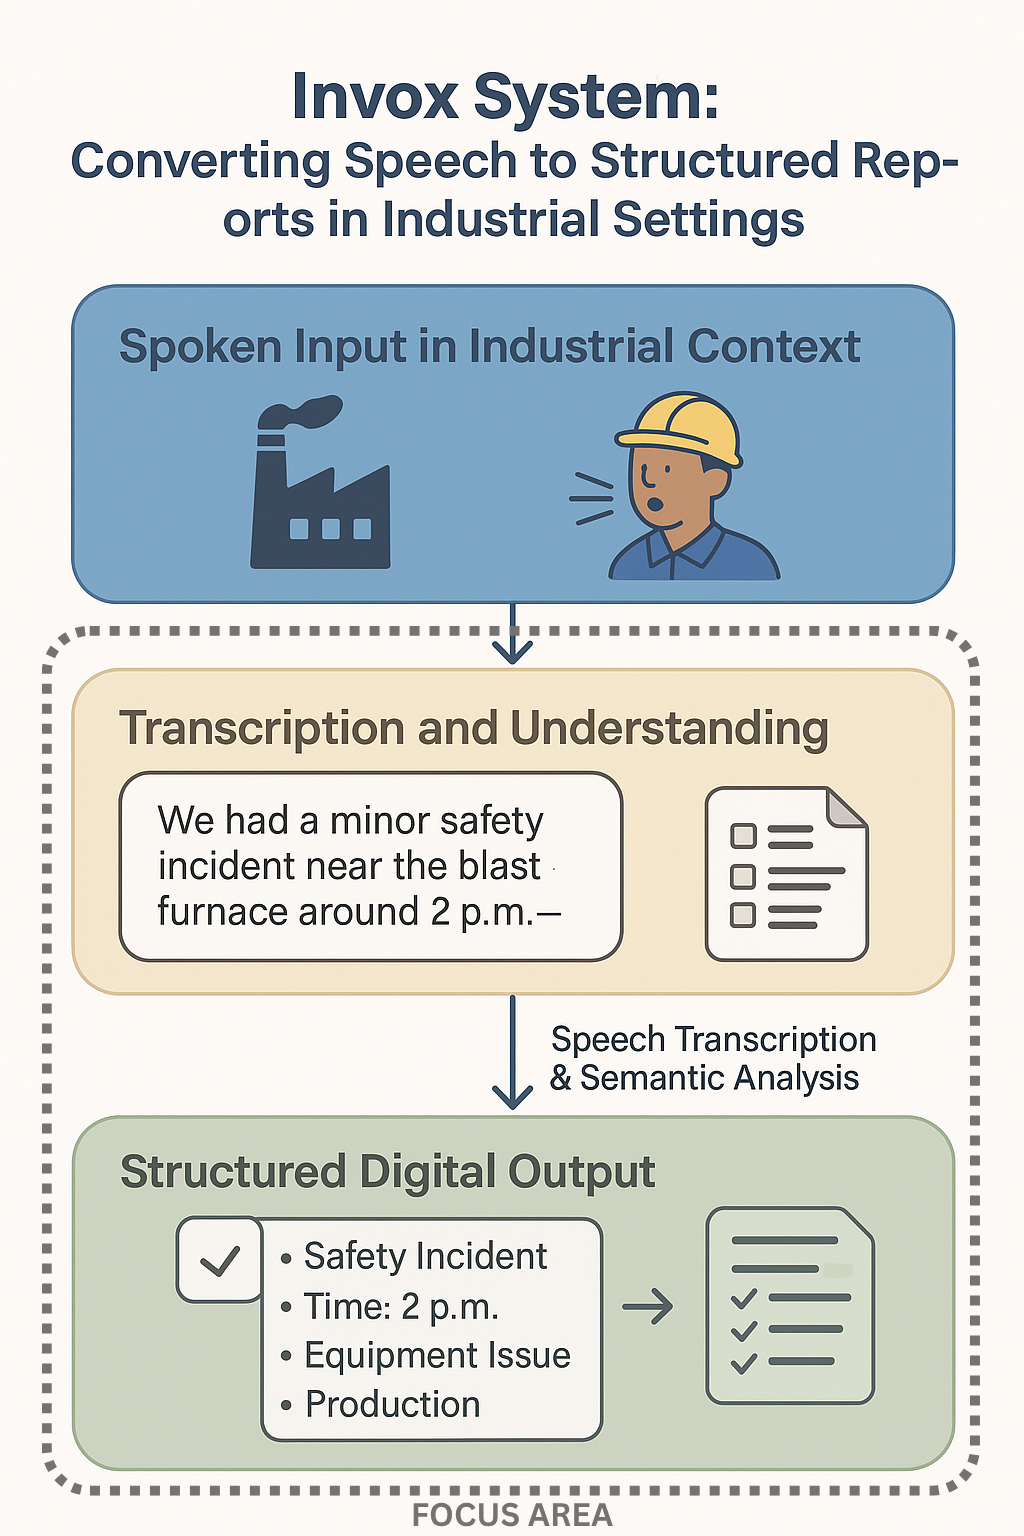
\includegraphics[scale=0.35]{images/Motivation.png}
    \caption{Invox: From spoken input to structured report}
    \label{fig:invox-motivation}
\end{figure}

Although this task may seem straightforward, it is far from trivial. Spoken input is often informal, unordered, and filled with vague expressions or filler words. Terms like “blast furnace” or “Line B” reflect domain-specific knowledge that the system must understand. Noise, fatigue, and rushed speech introduce further variability.

This scenario reveals four core challenges:
\begin{itemize}
    \item \textbf{Unstructured input:} Workers speak naturally, not in pre-defined templates.
    \item \textbf{Domain-specific language:} Technical terms and abbreviations must be recognized and interpreted.
    \item \textbf{Variability and noise:} Inconsistent phrasing, ambient noise, and disfluencies degrade transcription quality.
    \item \textbf{Template diversity:} Different departments use different reporting formats and vocabularies.
\end{itemize}

Together, these challenges underscore the need for a more intelligent and adaptable approach. A modular system like \textbf{Invox}, capable of processing speech, identifying relevant fields, and generating structured output, offers a scalable solution tailored to the complexities of real industrial environments.


\section{Scope of the Thesis}

This thesis is situated at the intersection of speech processing and natural language understanding, focusing on the task of converting noisy, unstructured spoken input into structured digital forms using large-scale pretrained models.

The primary use case addressed is shift documentation in the steel manufacturing industry. Operators in this domain often record verbal summaries at the end of their shifts, describing production events, safety incidents, and equipment issues. These recordings are typically informal, multilingual, and captured in noisy environments. This makes the use case ideal for evaluating robustness in low-structure, real-world input scenarios~\cite{wang2021spoken, fathullah2023prompting}.

The technical scope of this work includes the use of state-of-the-art automatic speech recognition (ASR) models—specifically OpenAI's Whisper~\cite{radford2023whisper}—combined with large language models (LLMs) such as GPT-5, Gemini-2.5-pro, etc. These components are orchestrated in a modular agent-based architecture for handling tasks like transcription interpretation, field-value mapping, and validation. No fine-tuning or training of models is performed; the focus is on system-level orchestration and domain-adapted prompt engineering.

The evaluation is limited to the accuracy and reliability of the structured output produced from recorded input. This thesis does not cover areas such as UI/UX design, live streaming input, conversational turn-taking, or the deployment of on-device inference. Instead, it aims to explore how existing ASR and LLM technologies can be effectively combined into a practical and scalable speech-based form filling system suitable for high-noise industrial domains.


\section{Objectives}

The main objective of this thesis is to design and evaluate a modular system—called \textbf{Invox}—that can automatically fill out structured forms using unstructured speech or text input. The system aims to overcome the limitations of current single-model, end-to-end solutions by introducing a flexible, multi-agent approach that separates the task into smaller, specialized components.

To achieve this goal, the following two specific objectives are defined:

\begin{enumerate}
    \item \textbf{Design a modular multi-agent architecture} for template filling that separates the process into subtasks such as transcription, field detection, answer generation, and verification—each handled by a dedicated agent. This design supports flexibility, transparency, and domain adaptability. As part of this design, five distinct prompting strategies are implemented using large language models (LLMs), ranging from single-pass full-input methods to iterative multi-model consensus approaches. These strategies are chosen to reflect different trade-offs in accuracy, latency, cost, and interpretability.

    \item \textbf{Evaluate the system performance} using a hybrid strategy that combines standardized benchmarking and real-world testing. For benchmarking, the official MUC-4 evaluation protocol \cite{chinchor1992muc4} is applied, using slot-level precision, recall, and F1-score to compare structured information extraction. Finally, results from all prompting strategies are compared to identify the most effective architectural approach under various real-world conditions.
\end{enumerate}

These objectives guide the development and validation of a system that is not only technically sound but also practical and scalable in industrial settings.


\section{Document Outline}

Following this introduction, the thesis begins with a discussion of related work in the field. This includes an overview of existing systems for template filling, particularly those that use speech input or large language models. The literature is analyzed to identify current limitations and to derive a clear set of requirements for building a better, more modular solution.

Next, the conceptual foundation of the proposed system is introduced. The structure of Invox is explained, along with four different design strategies that use large language models in distinct ways. These approaches are described in detail, along with the reasoning behind each one and a discussion of possible alternatives.

After outlining the concept, the implementation is described. This includes the software architecture, technology choices, and how each component—such as speech transcription, RAG, field extraction, and answer verification—was built. Attention is given to how modularity was achieved to support maintainability and reuse.

The following part of the thesis presents the working prototype. Screenshots, mockups, and usage examples are used to demonstrate how the system operates in practice. The user interface and interactions are shown, illustrating how speech input can be turned into a structured form with minimal effort.

Once the system is introduced and demonstrated, the evaluation section presents a detailed analysis of its performance. A benchmark dataset is used to test the system across four architectural approaches. The results are analyzed using metrics such as accuracy, latency, consistency, and computational cost.

The final part of the thesis summarizes the key findings, reflects on the strengths and limitations of the current implementation, and proposes ideas for future research and system improvements.


\chapter{Analysis}
This chapter identifies the fundamental requirements for converting natural language into structured templates and critically examines existing approaches. The goal is to establish a systematic basis for evaluating current methods and to derive implications for the design of the proposed framework.

\section{Requirements}

This section outlines the core requirements that a system must fulfill to transform natural language input into structured templates with predefined fields. Such templates are widely used across domains, including healthcare (e.g., patient checklists), manufacturing (e.g., quality inspections), and logistics (e.g., delivery reports).

The primary goal of the system presented in this thesis, named Invox, is to support users in filling out these templates more easily, quickly, and accurately. Instead of using traditional tools like a mouse, keyboard, or touchscreen, users interact with the system using natural language. This input can be typed or spoken aloud—both are valid forms of unstructured data. However, it is important to note that voice-based input is just one way of using the system; the true innovation lies in how the system processes and understands natural human language and translates it into structured form data.

In a traditional setting, filling out templates can be tedious. Users must manually locate the correct form, understand what each field is asking for, and type in the responses one by one. This is not only time-consuming but also error-prone. Mistakes may happen due to misunderstandings, skipped fields, or inconsistent use of terminology. The system described in this thesis seeks to overcome these problems by using a multi-agent architecture that processes unstructured input and populates templates automatically using large language models (LLMs).

The motivation behind using LLMs is their strong ability to understand context, infer meaning from loosely structured inputs, and generalize across different domains. When a user gives a voice or text description, the LLMs can interpret what they are trying to say—even if the input is informal, non-linear, or incomplete—and determine how to map this information into the correct fields of a form. This enables users to interact with the system in a more natural and efficient way.

However, building such a system is not straightforward. Several challenges must be addressed to ensure the solution is usable, reliable, and trustworthy across real-world scenarios. To clearly define what such a system should achieve, we identify the following six requirements:   

\textbf{R1 – Consistency:}  
The system must be able to transform heterogeneous and informal input—such as voice transcriptions, chat messages, or handwritten notes—into consistently populated template fields. It should normalize wording, tonality, length, and semantic specificity, and enforce formatting standards so that entries are comparable, unambiguous, and suitable for downstream analysis.  

\textbf{R2 – Information Extraction Abilities:}  
The system should accurately identify and assign relevant details from noisy, fragmented, or multilingual input to the correct fields, while leaving irrelevant fields empty. It must recognize when required information is missing, handle contradictions by prompting for clarification, and integrate scattered fragments into coherent entries.  

\textbf{R3 – Transparency:}  
To foster trust and accountability, the system must make its decision-making process visible. It should highlight the input fragments that support each extracted value and provide confidence scores to indicate the certainty of those values. This enables users to verify outputs efficiently, focus on uncertain cases, and ensure auditability in regulated domains.  

\textbf{R4 – User Correction:}  
The system must enable users to manually edit automatically populated template fields. This ensures immediate error resolution without requiring retraining and empowers users with direct control over the accuracy of the final data submitted.  

\textbf{R5 – Learning and Adaptation:}  
The system should improve over time by consolidating knowledge from past interactions and domain resources. It must learn from manually filled or corrected templates as well as from structured sources such as ontologies, glossaries, or rule sets, progressively reducing repetitive errors and improving alignment with domain-specific practices.

\textbf{R6 – Usability:}  
The system must deliver prompt, near–real-time feedback so interaction feels natural and uninterrupted. This requirement applies to both spoken and typed input (speech is only one use case). Usability is evaluated via end-to-end latency and must be interpreted relative to the declared hardware and deployment profile (e.g., GPU/TPU vs.\ CPU-only, concurrency, network).

These six requirements were identified based on the challenges discussed in Chapter 1 and are supported by current trends in research on natural language processing, speech and text interfaces, and intelligent form-filling systems. Each of the following sections will examine one requirement in detail. We explain what the requirement means, why it matters, and illustrate it with examples. For each requirement, we also define assessment standards that help evaluate how well the system satisfies the requirement in practice.  

\begin{figure}[h!]
    \centering
    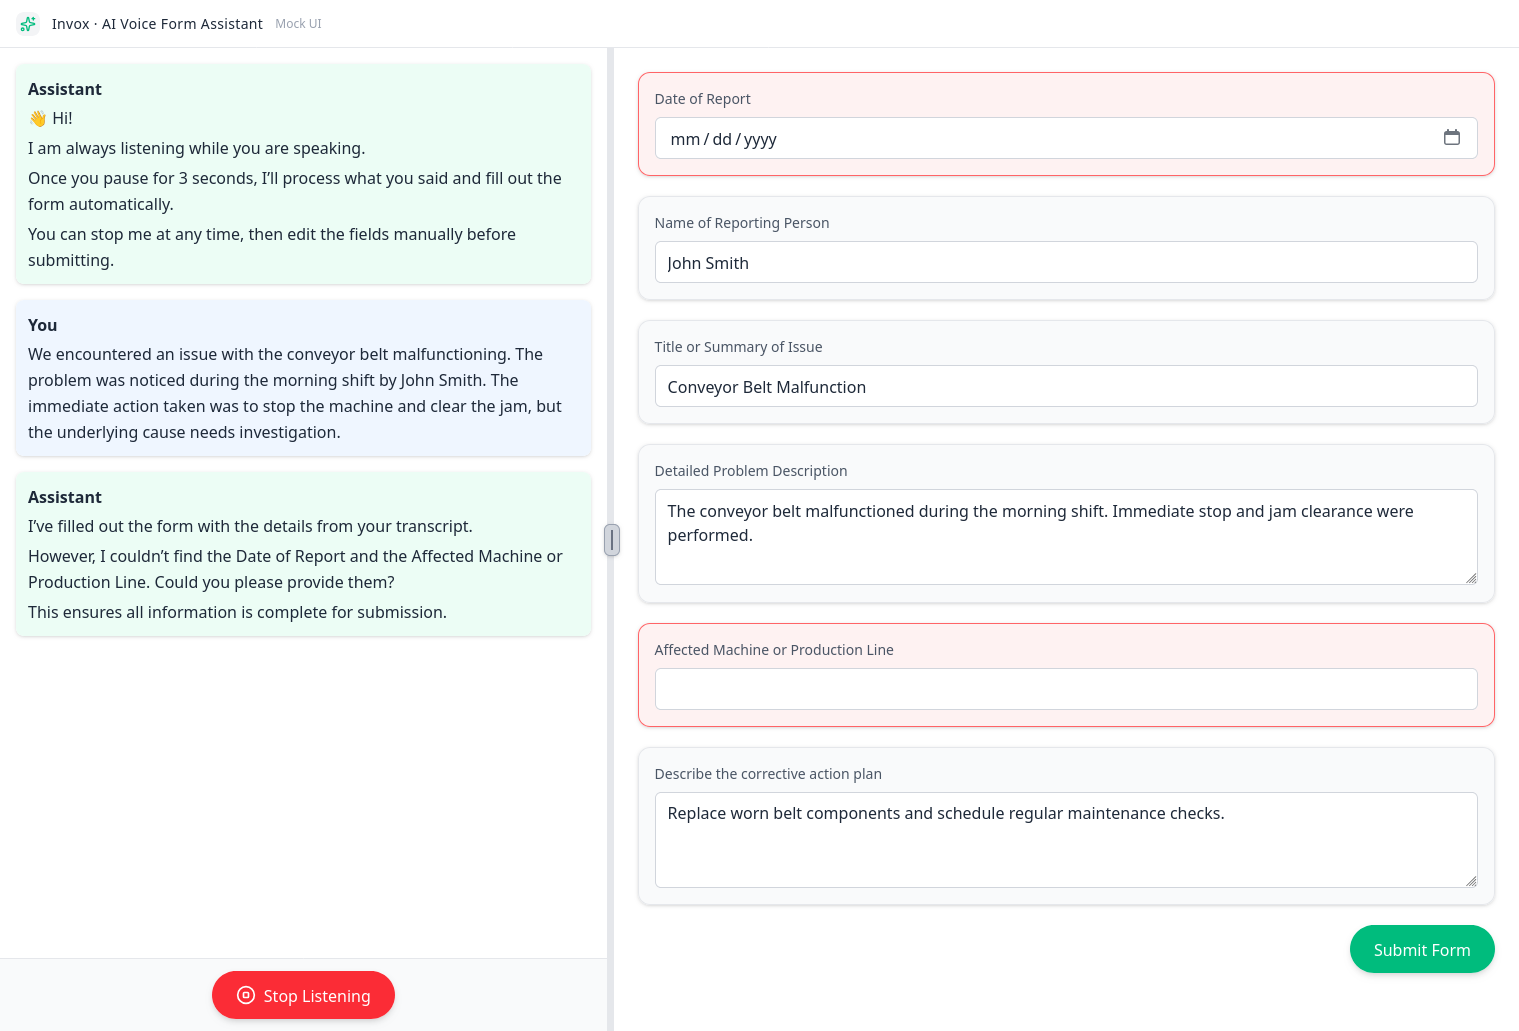
\includegraphics[width=\textwidth]{images/form-filling-example.png}
    \caption{Illustration of the form-filling framework. }
    \label{fig:form-filling-example}
\end{figure}


To make these requirements more concrete, Figure~\ref{fig:form-filling-example} shows a practical usage scenario of the Invox framework. On the left, the user provides a natural language description, which the assistant processes into a structured template on the right. Some fields are automatically filled with extracted values, while others remain highlighted as incomplete and require user clarification. This illustration highlights the central challenges addressed by the requirements: ensuring consistent representation of entries (R1), accurately extracting relevant details (R2), providing transparency about what was filled and why (R3), enabling user correction of missing or incorrect fields (R4), creating a foundation for gradual learning and adaptation over time (R5), and maintaining responsiveness so updates appear promptly during interaction (R6).

\subsection{R1: Consistency}
Consistency refers to the framework’s ability to transform heterogeneous and unstructured inputs—such as transcribed voice recordings, instant messages between employees, or informal written notes—into uniformly populated templates. Unlike free-text logs, templates require values that are standardized and comparable. This means that field entries must not vary arbitrarily in their wording, style, length, or level of specificity. This is a core aspect of what the research field calls "authorship attribution" in the context of LLMs, where the goal is to identify a consistent stylistic "fingerprint" from a given system~\cite{huang2024authorship}. Prior work in conversational systems has shown that a lack of normalization makes it difficult to align user inputs across contexts~\cite{liu2022conversational}, while studies in accessibility highlight how inconsistent representations reduce clarity and comparability for end users~\cite{clark2020accessible}. In the broader NLP field, research on natural language generation similarly stresses that variation without standardization complicates evaluation and downstream analysis~\cite{gatt2018survey}.


As illustrated in Figure~\ref{fig:form-filling-example}, an ideal solution should ensure that once information is extracted, the resulting field values are expressed in a consistent way. This means that answers are not only correct in content but also follow standardized wording, style, formatting, and level of detail. For example, dates should always appear in the same format, technical issues should be described with domain-specific terminology rather than colloquial phrasing, and descriptive fields should provide comparable levels of detail. Such uniform rendering makes entries easier to interpret for humans and more reliable to process automatically across different users, departments, or time periods.


This requirement is especially critical because heterogeneous sources of input inevitably produce inconsistent outputs if left unchecked. In industrial contexts, for example, one technician might describe a machine malfunction as a “slight issue,” another as a “minor fault,” and a third as a “mechanical malfunction.” Even if these phrases describe the same problem, their inconsistency complicates automated reporting and trend analysis, a challenge widely recognized in studies on data quality for industrial systems~\cite{norman2013design}. In healthcare, freeform reports such as “bad cough,” “patient has a cold,” or “respiratory illness” may all refer to the same condition. Medical informatics research has long emphasized that without concept normalization, such variations remain scattered as distinct entries and undermine clinical decision support~\cite{friedman2004survey}. More recent work on clinical text processing shows that mapping expressions to standardized terminologies is essential for interoperability and regulatory compliance~\cite{jonnalagadda2010medical, bodenreider2004unified}. Consistency therefore ensures that all such inputs are aligned to a common representational standard, enabling both human readability and machine-actionable analysis~\cite{shneiderman2016designing}.


In practice, consistency operates across multiple dimensions of representation. At the level of wording, normalization ensures that common phrases are mapped to standardized terminology. For example, “the patient has a cold” can be rendered as “patient with acute nasopharyngitis,” while “the thing is overheating” may be reformulated as “machine component exceeds temperature threshold.” At the level of tonality, consistency harmonizes register and style, replacing subjective or vague expressions such as “slight issue with machine” with standardized formulations such as “minor mechanical malfunction.” At the level of length, overly short entries like “headache” are enriched with sufficient detail to be meaningful, while excessively long descriptions such as “patient reports persistent mild headache for the past two days” are normalized into concise but precise formulations. Finally, at the semantic level, consistency promotes appropriate specificity, ensuring that generic categories like “illness” are consistently replaced with precise terms such as “influenza type B.”  

Formatting and style conventions are equally important to this requirement. Inconsistent formatting creates unnecessary barriers to readability and analysis. For instance, date entries should adhere to predefined standards so that “August 16th” is consistently represented as “08/16/2025.” Similarly, identifiers such as machine codes, patient IDs, or regulatory classification numbers should always follow the same syntactic pattern. Without such formatting alignment, even correctly normalized content may remain ambiguous or unusable across systems. Consistency therefore extends beyond lexical normalization to include structural and formal conventions that guarantee uniformity across the entire template.  

The advantages of consistent template filling are multifold. Consistency improves readability, as users can process and compare entries more quickly when values follow uniform patterns of wording and formatting. It reduces ambiguity by replacing vague or stylistically divergent expressions with precise, standardized equivalents, thereby lowering the risk of misunderstanding. It increases the usefulness of templates in professional contexts, ensuring that field entries are sufficiently detailed to meet regulatory, diagnostic, or legal requirements. Finally, it enhances comparability: homogeneous field values are easier to query, index, and aggregate, which facilitates automated reporting and large-scale data analysis across organizations and timeframes. 

\begin{table}[h!]
\centering
\renewcommand{\arraystretch}{1.6}
\setlength{\tabcolsep}{12pt}
\begin{tabularx}{\textwidth}{|>{\centering\arraybackslash}m{3cm}|>{\arraybackslash}X|}
\hline
\textbf{Visual Score} & \textbf{Interpretation (with thresholds)} \\
\hline
\centering\raisebox{0pt}{\tikz[baseline]{\filldraw[fill=black] (0,0) circle (0.4cm);}} 
& \textbf{High consistency.} Structured fields are correct in most cases (macro exact match/F1 $\geq 0.80$), and free-text fields show strong semantic and stylistic alignment (normalized BLEURT $\geq 0.70$ and Cosine Similarity $\geq 0.70$). \\
\hline
\centering\raisebox{0pt}{\tikz[baseline]{\filldraw[fill=black] (0,0) -- (90:0.4cm) arc (90:-150:0.4cm) -- cycle; \draw (0,0) circle (0.4cm);}} 
& \textbf{Medium consistency.} Structured fields show moderate accuracy (macro exact match/F1 in $[0.65, 0.80)$), and free-text fields achieve moderate semantic and stylistic similarity (normalized BLEURT in $[0.55, 0.70)$ and Cosine Similarity in $[0.55, 0.70)$). \\
\hline
\centering\raisebox{0pt}{\tikz[baseline]{\filldraw[fill=black] (0,0) -- (90:0.4cm) arc (90:-30:0.4cm) -- cycle; \draw (0,0) circle (0.4cm);}} 
& \textbf{Low consistency.} Structured fields are often incorrect (macro exact match/F1 in $[0.50, 0.65)$), and free-text fields align poorly (normalized BLEURT in $[0.40, 0.55)$ and Cosine Similarity in $[0.40, 0.55)$). \\
\hline
\centering\raisebox{0pt}{\tikz[baseline]{\draw (0,0) circle (0.4cm);}} 
& \textbf{No consistency.} Structured accuracy is very low (macro exact match/F1 $<0.50$) and free-text similarity is weak (normalized BLEURT $<0.40$ and Cosine Similarity $<0.40$). Entries are unreliable for comparison or analysis. \\
\hline
\end{tabularx}
\caption{Evaluation scale for R1: Consistency.}
\label{tab:r1-consistency-thresholds}
\end{table}

For evaluation, we use exact match or F1 scores on structured fields such as identifiers, categories, and dates, and BLEURT on free-text fields such as descriptions or notes. Because raw BLEURT scores can vary depending on the checkpoint and dataset, we normalize them to $[0,1]$ across all system outputs in the test set.

To further evaluate the consistency of the system's output style—a key challenge in LLM-generated text—we also employ a stylometric analysis. Specifically, we measure the Cosine Similarity of the n-gram distributions between each system's output and the golden benchmark. Unlike Jaccard similarity, which only considers the presence or absence of n-grams, Cosine Similarity accounts for their frequency. N-grams, which are contiguous sequences of words, provide a quantitative measure of the system's syntactic style. A higher similarity score here indicates that the system's output is not only semantically correct (as measured by BLEURT) but also stylistically aligned with a human-authored standard, thus providing a more comprehensive evaluation of consistency.

To summarize, consistency ensures that heterogeneous, informal, or ambiguous user inputs are transformed into standardized, comparable, and semantically coherent template entries. By enforcing normalization across wording, tonality, length, semantic level, and formatting conventions, and by measuring agreement with the gold standard through exact match for structured fields and BLEURT for free-text fields, the system improves readability, minimizes ambiguity, and ensures that structured data can serve as a reliable foundation for both human decision-making and automated analysis.  
 

\subsection{R2: Information Extraction}
Information extraction refers to the framework’s ability to accurately identify and populate relevant template fields from unstructured or semi-structured input, while leaving irrelevant fields empty. This process goes beyond simple keyword matching and instead relies on linguistic context, entity relationships, and domain-specific semantics to ensure that extracted values are both accurate and meaningful~\cite{grishman1997information, sarawagi2008information}. In practice, information extraction determines whether heterogeneous and noisy inputs—such as partially transcribed voice recordings, multilingual text segments, or fragmented chat messages—can be transformed into reliable structured data~\cite{jurafsky2023speech, liu2022conversational}.  

As illustrated in Figure~\ref{fig:form-filling-example}, an ideal solution must be able to extract relevant details even when input is noisy, fragmented, or multilingual, and populate the corresponding template fields while leaving others empty. The highlighted gaps in the example show that extraction is not only about finding correct values but also about reliably detecting when information is missing and avoiding unsupported guesses.

This requirement matters because real-world text is rarely clean or complete. Voice transcriptions may drop words or introduce errors, employees in international environments may switch between languages mid-sentence, and workplace chat logs often contain fragments, abbreviations, or extraneous commentary~\cite{baldwin2013noisy}. Without strong extraction capabilities, systems risk either leaving critical fields blank or, worse, filling them with incorrect assumptions. In regulated or safety-critical domains such as healthcare or industrial maintenance, such errors can result in compliance violations, misdiagnoses, or operational risks~\cite{radford2023whisper, fathullah2023prompting}.  

Effective extraction must address several challenges simultaneously. First, it must be robust to mixed-language and incomplete input, requiring cross-lingual transfer capabilities for reliable extraction~\cite{ruder2019cross}. A report that states “der Patient… fever since yesterday” combines German and English, yet the system must still detect the symptom and correctly populate the appropriate field. Equally important is recognizing when essential details are missing and preserving empty fields instead of filling them with fabricated values. For example, if a date of inspection is not provided, the system should explicitly leave the field empty rather than guessing. Second, conflict handling is essential. If a transcript contains contradictory information—such as “appointment on August 10” followed by “meeting scheduled for August 12”—the system should not arbitrarily choose one date. Instead, it must detect the inconsistency and prompt the user for clarification, ensuring reliability of the final record. Third, extraction requires contextual understanding. Information is often scattered across multiple parts of a conversation or document, and the system must combine relevant fragments into coherent field values while ignoring unrelated chatter. For instance, if a technician states, “We restarted the press at 23:14. Oh, and the noise got louder after ten minutes,” the system must connect these details to the same inspection event rather than treating them as separate or unrelated entries.  

\begin{table}[h!]
\centering
\renewcommand{\arraystretch}{1.6}
\setlength{\tabcolsep}{12pt}
\begin{tabularx}{\textwidth}{|>{\centering\arraybackslash}m{3cm}|>{\arraybackslash}X|}
\hline
\textbf{Visual Score} & \textbf{Interpretation (based on criteria)} \\
\hline
\centering\raisebox{0pt}{\tikz[baseline]{\filldraw[fill=black] (0,0) circle (0.4cm);}} 
& \textbf{All three criteria satisfied.} The system reliably handles mixed-language and incomplete text, correctly detects and flags conflicts, and successfully integrates related information spread across different text parts. \\
\hline
\centering\raisebox{0pt}{\tikz[baseline]{\filldraw[fill=black] (0,0) -- (90:0.4cm) arc (90:-150:0.4cm) -- cycle; \draw (0,0) circle (0.4cm);}} 
& Two criteria satisfied. For instance, the system handles mixed-language input and detects conflicts but fails to integrate scattered contextual information. \\
\hline
\centering\raisebox{0pt}{\tikz[baseline]{\filldraw[fill=black] (0,0) -- (90:0.4cm) arc (90:-30:0.4cm) -- cycle; \draw (0,0) circle (0.4cm);}} 
& One criterion satisfied. For instance, the system handles mixed-language and incomplete text but fails to detect conflicts and integrate contextual information. \\
\hline
\centering\raisebox{0pt}{\tikz[baseline]{\draw (0,0) circle (0.4cm);}} 
& No criteria satisfied. The system fails to handle mixed-language input, cannot detect conflicts, and does not integrate information spread across different parts of the input. \\
\hline
\end{tabularx}
\caption{Evaluation Scale for R2: Information Extraction Abilities.}
\label{tab:r2-extraction-metrics}
\end{table}


The advantages of strong information extraction capabilities extend across multiple dimensions. They improve accuracy by minimizing both incorrect and missing field values, even when input is fragmented or linguistically complex. They reduce user workload by lowering the amount of manual correction required after automatic field population. They enhance robustness to noise by maintaining performance in the presence of typos, filler words, or irrelevant side remarks. Finally, they enable better multi-source integration by combining relevant information from different segments into a single coherent template entry, which is particularly valuable in collaborative or multi-turn interactions~\cite{shneiderman2016designing}.  

To summarize, information extraction abilities determine whether heterogeneous and noisy user inputs can be reliably transformed into structured templates. A robust system not only identifies and assigns relevant details but also recognizes gaps, resolves contradictions, and integrates scattered fragments into coherent entries. This reduces user workload, improves reliability, and ensures that the extracted data supports both operational decision-making and automated analysis.
 

\subsection{R3: Transparency}
Transparency refers to the framework’s ability to make its decision-making process visible to users by exposing both the evidence behind each extracted value and the system’s level of certainty in that value. Unlike black-box systems that present outputs without explanation, a transparent framework not only shows the populated fields but also reveals the reasoning path by which they were derived. This includes identifying the input fragments that served as evidence and providing explicit indicators of how confident the system is in its interpretations~\cite{doshi2017towards, samek2019explainable}.  

As illustrated in Figure~\ref{fig:form-filling-example}, transparency in an ideal framework means that populated values are never shown in isolation but are accompanied by their supporting evidence and a confidence indicator. The figure highlights how a field such as a date is linked back to the exact phrase in the transcript and annotated with a certainty level, making the reasoning process visible rather than opaque.

This requirement matters because users often interact with template filling systems in high-stakes environments where correctness cannot be taken for granted. In domains such as healthcare, industrial inspection, or compliance reporting, an incorrectly extracted date, measurement, or symptom could lead to operational errors or legal consequences. Without transparency, users are left to either blindly trust the system or manually re-check all outputs. Both outcomes undermine efficiency and adoption. By contrast, when the system highlights the origin of each extracted field and communicates its confidence level, users can selectively verify uncertain or ambiguous entries, thereby improving both trust and productivity~\cite{wang2022trust, ribeiro2016should}.  

In practice, transparency is achieved through two complementary mechanisms. First, source highlighting makes explicit which text fragments in the input led to the population of a given field. For instance, if the transcript contains the phrase “scheduled for 08/16/2025,” the system should highlight this fragment as the evidence for the “Date” field. This allows users to directly trace values back to their textual origins and verify their correctness. Second, confidence scores quantify the system’s certainty about each extracted value. These can be expressed as probabilities (e.g., 0.82 confidence in the extracted date) or as categorical levels (e.g., high, medium, low). Confidence scores help users prioritize where to invest their attention, focusing on entries that are most likely to contain errors while trusting those that are more secure. Together, these mechanisms turn opaque predictions into traceable, verifiable decisions.  

The advantages of transparency are multifold. It builds user trust by establishing a clear link between input data and structured outputs, reducing the perception of the system as a “black box.” It enables efficient error detection, since users can quickly locate uncertain or weakly supported values without re-checking the entire template. Transparency also facilitates training and feedback, as developers and domain experts can identify systematic error patterns by examining low-confidence predictions and their sources~\cite{thomas2019interacting}. Finally, transparency supports compliance in regulated industries by providing auditable evidence trails that show not only what the system decided but also why it decided it.  

\begin{table}[h!]
\centering
\renewcommand{\arraystretch}{1.6}
\setlength{\tabcolsep}{12pt}
\begin{tabularx}{\textwidth}{|>{\centering\arraybackslash}m{3cm}|>{\arraybackslash}X|}
\hline
\textbf{Visual Score} & \textbf{Interpretation} \\
\hline
\centering\raisebox{0pt}{\tikz[baseline]{\filldraw[fill=black] (0,0) circle (0.4cm);}} 
& \textbf{Both criteria satisfied.} The system highlights the exact text fragments that led to each populated field and provides confidence scores for all extracted values. \\
\hline
\centering\raisebox{0pt}{\tikz[baseline]{\filldraw[fill=black] (0,0) -- (90:0.4cm) arc (90:-90:0.4cm) -- cycle; \draw (0,0) circle (0.4cm);}} 
& One criterion satisfied (e.g., confidence scores are displayed but no source highlighting is provided, or vice versa). \\
\hline
\centering\raisebox{0pt}{\tikz[baseline]{\draw (0,0) circle (0.4cm);}} 
& No criteria satisfied. The system provides populated fields without indicating their source or the certainty of extraction, leaving the process opaque. \\
\hline
\end{tabularx}
\caption{Evaluation Scale for R3: Transparency}
\label{tab:r3-transparency}
\end{table}

To summarize, transparency ensures that extracted template values are not only presented as results but also explained in terms of their origins and associated confidence levels. By exposing the reasoning process, the system strengthens user trust, enables efficient verification, and provides the auditability necessary for both iterative improvement and compliance in regulated domains.
 

\subsection{R4: User Correction}
User correction refers to the framework’s ability to allow manual modifications of populated template fields after automatic extraction has taken place. Unlike automated adaptation mechanisms, which rely on system learning from prior interactions, user correction focuses on immediate, explicit interventions that ensure the accuracy of individual outputs. It grants end-users direct control over the final contents of a template, ensuring that errors in recognition, interpretation, or formatting can be addressed before the data is finalized~\cite{bohus2005sorry, shneiderman2016designing}.  

As illustrated in Figure~\ref{fig:form-filling-example}, an ideal framework must let users directly modify any field highlighted as incorrect or uncertain. The figure shows how entries flagged by the system can be overwritten or adjusted before finalization, ensuring that human judgment always has the final word in the template.

This requirement matters because no automated extraction system can achieve perfect accuracy across all input conditions. Transcriptions may introduce errors, ambiguous phrases may be misinterpreted, and domain-specific terminology may be inconsistently mapped. In practical contexts such as medical documentation or maintenance inspections, even small inaccuracies—such as recording the wrong date of an incident or misreporting a measurement—can have disproportionate consequences. By enabling users to directly edit system-generated values, frameworks ensure that such errors can be corrected in real time without the need for retraining, secondary workflows, or downstream data cleaning~\cite{norman2013design}.  

In practice, correction functionality should be applied at the field level. Users must be able to select any automatically populated entry and replace it with the intended value, for example correcting “08/16/2025” to “08/15/2025” in a date field or updating “mechanical failure” to “electrical failure” in an inspection log. Such capabilities not only resolve errors but also give users confidence in the system by demonstrating that the outputs are not immutable black-box predictions. This aligns with broader human–computer interaction principles emphasizing user empowerment, flexibility, and control over system outputs~\cite{shneiderman2016designing, hoy2018voice}.  

The advantages of user correction are twofold. First, it enables immediate error resolution: users do not need to wait for iterative model updates or retraining cycles to address mistakes, but can directly ensure accuracy within the current interaction. Second, it promotes user empowerment by giving individuals ownership of the final data submitted, strengthening their trust in the system and reducing frustration when mistakes inevitably occur. These benefits are particularly important in time-sensitive workflows, where operators must finalize records quickly while retaining the ability to guarantee correctness~\cite{amershi2019guidelines}.


\begin{table}[h!]
\centering
\renewcommand{\arraystretch}{1.6}
\setlength{\tabcolsep}{12pt}
\begin{tabularx}{\textwidth}{|>{\centering\arraybackslash}m{3cm}|>{\arraybackslash}X|}
\hline
\textbf{Visual Score} & \textbf{Interpretation} \\
\hline
\centering\raisebox{0pt}{\tikz[baseline]{\filldraw[fill=black] (0,0) circle (0.4cm);}} 
& \textbf{Full correction support.} Users can edit any populated field directly, ensuring complete control over the final template. \\
\hline
\centering\raisebox{0pt}{\tikz[baseline]{\draw (0,0) circle (0.4cm);}} 
& \textbf{No correction support.} Automatically populated values cannot be modified by users, leaving inaccuracies unresolved. \\
\hline
\end{tabularx}
\caption{Evaluation Scale for R4: User Correction}
\label{tab:r4-correction}
\end{table}

To summarize, user correction ensures that populated templates remain accurate by enabling individuals to directly edit extracted values. This requirement emphasizes immediate error resolution and user empowerment, giving people control over final outputs while reinforcing trust in the system’s reliability.


\subsection{R5: Learning and Adaptation}
Learning and adaptation refer to the framework’s ability to improve its performance over time by incorporating knowledge from user interactions, corrections, and structured domain information. Unlike static systems, which produce the same outputs regardless of experience, an adaptive framework evolves continuously. It refines its internal models and decision-making strategies based on provided examples, explicit corrections, and formal domain rules, thereby becoming more accurate and contextually aligned with the environment in which it is deployed~\cite{doshi2017towards, sun2023slot}.  

As illustrated in Figure~\ref{fig:form-filling-example}, finalized corrections and domain glossaries feed a feedback loop that informs future fills. This matters because using both sources reduces recurring errors and steadily improves accuracy.

This requirement matters because template filling systems are often deployed in highly specialized settings where general-purpose models cannot fully capture local terminology, workflows, or conventions. For example, a healthcare provider may require specific mappings between colloquial expressions such as “chest cold” and formal diagnostic categories, while a manufacturing plant may use internal identifiers or shorthand that differ from industry-wide terminology. Without learning and adaptation, the system risks repeating the same mistakes indefinitely, requiring users to make the same corrections again and again. By contrast, a system that consolidates knowledge from past interactions and domain inputs progressively reduces error rates and builds long-term efficiency~\cite{liu2022conversational, mialon2023augmented}.  

In practice, adaptation can occur through two complementary mechanisms. First, learning from provided filled-in templates allows the system to build expectations about the type and structure of values that belong in each field. For example, if historical forms consistently show that an employee ID consists of exactly five characters, the system can detect when a user provides only three and prompt them to complete the entry correctly. Over time, such feedback reduces recurring formatting or completeness errors by aligning new inputs with established patterns. Second, learning from domain knowledge integrates structured resources such as ontologies, glossaries, or formal rule sets. For instance, a medical ontology may specify that “flu” and “influenza” are synonymous terms, while an engineering glossary may define acceptable formats for torque values. By encoding such knowledge, the system improves both extraction and formatting, aligning outputs with established standards rather than ad-hoc interpretations~\cite{clark2020accessible, chen2024webforms}.

The advantages of learning and adaptation are cumulative. Accuracy improves progressively as the system incorporates examples and corrections, ensuring that the framework becomes more reliable the longer it is used in a given domain. Knowledge consolidation ensures that corrections made once benefit future cases, reducing the burden of repetitive manual adjustments. Continuous refinement also lowers the risk of systematic errors, as patterns of mistakes are gradually eliminated. These capabilities transform template filling from a static tool into an evolving system that adapts to organizational needs and grows more effective with sustained use~\cite{shneiderman2016designing, amershi2019guidelines}.  

\begin{table}[h!]
\centering
\renewcommand{\arraystretch}{1.6}
\setlength{\tabcolsep}{12pt}
\begin{tabularx}{\textwidth}{|>{\centering\arraybackslash}m{3cm}|>{\arraybackslash}X|}
\hline
\textbf{Visual Score} & \textbf{Interpretation} \\
\hline
\centering\raisebox{0pt}{\tikz[baseline]{\filldraw[fill=black] (0,0) circle (0.4cm);}} 
& \textbf{Both mechanisms satisfied.} The system learns from corrected or manually filled templates and incorporates structured domain knowledge such as ontologies and glossaries. \\
\hline
\centering\raisebox{0pt}{\tikz[baseline]{\filldraw[fill=black] (0,0) -- (90:0.4cm) arc (90:-90:0.4cm) -- cycle; \draw (0,0) circle (0.4cm);}} 
& One mechanism satisfied (e.g., the system learns from corrections but cannot integrate domain knowledge, or vice versa). \\
\hline
\centering\raisebox{0pt}{\tikz[baseline]{\draw (0,0) circle (0.4cm);}} 
& No mechanisms satisfied. The system is static, with no ability to learn from past usage or structured knowledge sources. \\
\hline
\end{tabularx}
\caption{Evaluation Scale for R5: Learning and Adaptation}
\label{tab:r5-learning}
\end{table}

To summarize, learning and adaptation ensure that the framework evolves with use, incorporating both user-provided corrections and structured domain knowledge. This capability reduces repetitive errors, consolidates expertise, and progressively improves accuracy, enabling the system to remain aligned with the specialized needs of its deployment context.


\subsection{R6: Usability}
\subsection*{R6: Usability}

Usability in the context of this framework refers primarily to \textbf{latency}, i.e., the time delay between user input and the system’s output (e.g., updated template fields becoming visible). While this thesis evaluates a speech-driven scenario, \emph{speech is only one use case}; the core task is the transformation of \emph{unstructured input (spoken or typed text)} into structured templates. Accordingly, the latency requirement applies to any unstructured-to-template pipeline (typed submissions, transcripts, or mixed modalities). In such settings, responsiveness directly determines whether interaction feels natural and uninterrupted. Human–computer interaction research consistently shows that feedback within two to three seconds is perceived as natural turn-taking, while longer delays disrupt concentration and diminish trust in the system~\cite{shneiderman2016designing}. For voice-first applications, user expectations are shaped by everyday experiences with assistants, where near-instantaneous responses are the norm~\cite{wang2021slu}.

As illustrated in Figure~\ref{fig:form-filling-example}, the template should update promptly after a spoken or typed submission. Timely visual feedback preserves flow and enables quick verification.

Unlike accuracy or error tolerance, which are covered in other requirements (R1–R5), usability here is scoped strictly to latency. This requirement matters because template filling often occurs in time-pressured contexts (e.g., hospitals or industrial facilities), where long waiting times interrupt workflows. For example, a technician dictating a machine fault—or a clerk pasting a long free-text note—must continue seamlessly; if the system takes ten or more seconds to update, the reporting process is disrupted and efficiency drops. Thus, latency is the decisive factor for adoption in real-world deployments.

However, latency is not an absolute property of the software alone. It is strongly influenced by the \textbf{hardware and deployment environment} on which inference is performed. High-performance accelerators such as GPUs and TPUs can significantly reduce end-to-end response time, whereas CPU-only or resource-constrained devices typically increase delays~\cite{shneiderman2016designing, jurafsky2023slp}. Therefore, when evaluating usability, latency benchmarks must always be reported together with the hardware profile (e.g., GPU/TPU type, number of concurrent users, and network setting). This ensures that usability scores are interpreted relative to realistic deployment contexts rather than as abstract performance claims.

\begin{table}[h!]
\centering
\renewcommand{\arraystretch}{1.6}
\setlength{\tabcolsep}{12pt}
\begin{tabularx}{\textwidth}{|>{\centering\arraybackslash}m{3cm}|>{\arraybackslash}X|}
\hline
\textbf{Visual Score} & \textbf{Interpretation} \\
\hline
\centering\raisebox{0pt}{\tikz[baseline]{\filldraw[fill=black] (0,0) circle (0.4cm);}} 
& \textbf{High usability.} p95 end-to-end (E2E) latency $\leq$ 3\,s on the declared hardware profile. Interaction feels natural; conversational pacing is preserved. \\
\hline
\centering\raisebox{0pt}{\tikz[baseline]{\filldraw[fill=black] (0,0) -- (90:0.4cm) arc (90:-90:0.4cm) -- cycle; \draw (0,0) circle (0.4cm);}}
& \textbf{Medium usability.} p95 E2E latency in $(3,10)$\,s. Delay is noticeable but tolerable in most workflows. \\
\hline
\centering\raisebox{0pt}{\tikz[baseline]{\draw (0,0) circle (0.4cm);}} 
& \textbf{No usability.} p95 E2E latency $>$ 10\,s or frequent timeouts. Workflow is impractical under this configuration. \\
\hline
\end{tabularx}
\caption{Evaluation Scale for R6: Usability}
\label{tab:r6-usability}
\end{table}

\paragraph{Evaluation method (latency definition).}
We measure \emph{end-to-end (E2E) latency} from the time the user finishes an utterance \emph{or submits text} until the corresponding template fields are rendered. For each system, p95 latency is reported (optionally p50 for typical-case summaries), ensuring responsiveness is captured consistently~\cite{amershi2019guidelines, jurafsky2023slp}. All results must specify the underlying hardware setup.

To summarize, usability in this framework is defined as responsiveness measured through latency for unstructured-to-template conversion across modalities (speech and text). Because latency is hardware-dependent, evaluation must always contextualize results by reporting the target infrastructure. This ensures comparability across systems while keeping interpretations grounded in practical deployment realities.



\section{Related Work}

The transformation of unstructured natural language into structured templates represents a fundamental challenge in natural language processing that intersects multiple research domains. This challenge has gained renewed attention with the advent of large language models (LLMs), which demonstrate unprecedented capabilities in understanding context, extracting relevant information, and generating structured outputs from free-form text. 

However, despite these advances, current approaches often struggle with the specific requirements identified in Section 2.1, particularly when dealing with noisy, domain-specific, or incomplete inputs common in real-world industrial and professional settings.
This section examines the current state of research relevant to multi-agent template filling systems, with particular focus on how existing approaches address the core challenges of consistency, information extraction accuracy, transparency, user correction capabilities, learning mechanisms, and usability. The analysis reveals significant gaps in current methodologies, particularly in their monolithic design assumptions and limited adaptability to specialized domains.

The review is organized into four key areas that directly inform the design of the proposed Invox system. First, we examine traditional and modern approaches to template filling and structured information extraction, tracing the evolution from rule-based systems to contemporary LLM-driven methods. Second, we analyze prompt engineering techniques that have emerged as critical tools for guiding LLMs toward structured output generation. Third, we explore multi-agent LLM systems that decompose complex tasks into specialized components, offering potential solutions to the modularity and transparency challenges identified in monolithic approaches. Finally, we evaluate how existing solutions perform against the six requirements established in this thesis, identifying specific limitations that motivate the need for a more comprehensive, modular approach to speech-driven template filling.


\subsection{Template Filling and Structured Information Extraction}
Extracting structured information from unstructured text has been a central challenge in natural language processing (NLP) for decades. Early systems were rule-based, using handcrafted grammars, dictionaries, and regular expressions to detect domain-specific patterns \cite{grishman1997information}. These methods worked well in narrow settings but were brittle, required heavy manual effort, and could not easily adapt to new domains.

Statistical models offered more flexibility. Hidden Markov Models (HMMs) were used to model sequential dependencies, while Conditional Random Fields (CRFs) became particularly influential by enabling richer feature-based sequence labeling \cite{sarawagi2008information}. CRFs were widely adopted for tasks such as Named Entity Recognition (NER) and slot filling, achieving strong results on shared tasks like CoNLL-2003 \cite{tjong2003introduction}. Despite these advances, statistical models still struggled with domain transfer, long-range dependencies, and their reliance on handcrafted features.

Another important limitation of early work was the reliance on pipeline-based architectures. Classical information extraction was usually divided into subtasks such as entity recognition, relation classification, and template alignment. Each stage depended on the output of the previous one, which often led to error propagation \cite{jurafsky2023speech}. For example, if the entity recognition module mislabeled an organization, that error would carry over to relation classification and template population. While pipelines offered modularity, they lacked robustness and transparency, making them hard to apply in noisy or domain-specific environments.

A major breakthrough came with the transformer architecture \cite{vaswani2017attention}. Transformers introduced self-attention and large-scale pretraining, which made it possible to capture long-range context and resolve ambiguity in ways earlier models could not. Building on this foundation, large language models (LLMs) can now generate structured outputs directly, for example in JSON, XML, or task-specific templates. This has enabled information extraction to be performed in zero-shot or few-shot settings, significantly reducing the need for task-specific labeled data \cite{brown2020language,wei2022emergent}. This marks a shift from extractive, pipeline-based designs to generative, end-to-end systems.

One influential contribution in this direction is the work of Du, Rush, and Cardie on \textit{Template Filling with Generative Transformers} \cite{du2021template}. Their framework replaces the traditional two-step pipeline of NER followed by event classification with a single generative system. The model conditions on document tokens and event type markers to generate slot fillers directly. This design captures dependencies across multiple events in one document, avoiding the error propagation typical of pipelines. On the MUC-4 dataset, their approach outperformed both pipeline-based and extractive neural baselines, especially for documents that described multiple events.

\begin{figure}
    \centering
    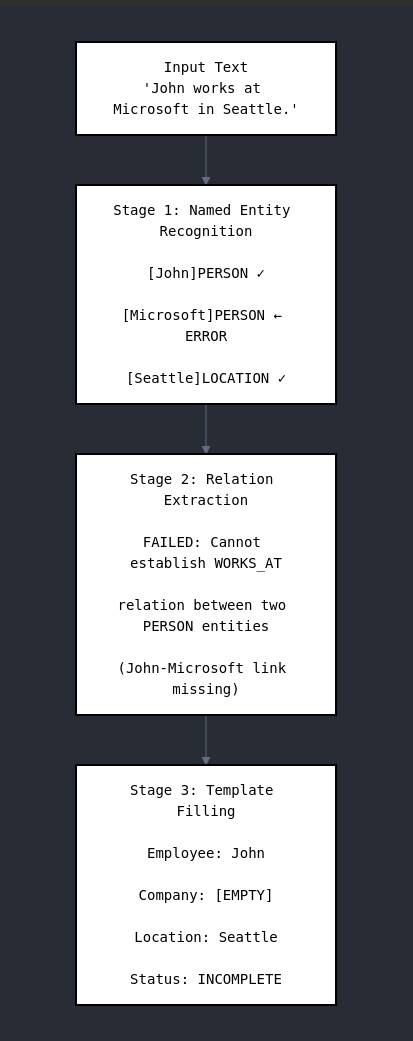
\includegraphics[width=0.6\linewidth]{images/error_propagation.png}
    \caption{Error Propagation Illustration}
    \label{fig:placeholder}
\end{figure}

Benchmarks have played a crucial role in driving research in this area. The MUC-4 dataset \cite{chinchor1992muc} defined an early template filling task for terrorism-related news reports. The ACE program \cite{doddington2004ace} expanded the scope by introducing entity, relation, and event extraction benchmarks across domains. CoNLL-2003 \cite{tjong2003introduction} provided a widely used benchmark for NER in English and German newswire. More recently, speech-based datasets such as SLURP \cite{bastianelli2020slurp} have enabled evaluation of spoken language understanding and slot filling. These benchmarks revealed both the strengths and weaknesses of successive methods, showing where statistical approaches failed and where generative models improved performance. However, they also highlighted the limitations of surface-level metrics such as precision, recall, and F1, which do not capture issues like consistency or robustness.

Despite these advances, domain-specific challenges remain. In healthcare, systems must handle specialized terminology, abbreviations, and implicit knowledge that may not be stated explicitly \cite{friedman2004survey}. In manufacturing and industrial contexts, extraction is complicated by technical identifiers, inconsistent documentation, and informal reporting styles often found in shift logs or maintenance notes \cite{wang2021slu}. These domains require systems that combine robustness with adaptability to diverse forms of domain language.

Work on speech-driven template filling has also emerged. Sun et al.\ study \textit{Speech-based Slot Filling using Large Language Models} \cite{sun2023slot}, focusing on the task of extracting slot values from automatic speech recognition (ASR) transcriptions under noisy conditions. Their evaluation of GPT-3.5, GPT-4, LLaMA, and Vicuna on the SLURP dataset introduces techniques such as structured prompt design, noise-robust LoRA fine-tuning, and linearised knowledge injection (LKI). Their findings show that while LLMs generalize well in zero-shot and few-shot settings, robustness in real-world speech requires careful prompt design and adaptation strategies. This is particularly relevant for this thesis, which addresses speech-based template filling.

Practical tools are also emerging. LangExtract, developed by Google, provides a schema-based information extraction framework using LLMs \cite{google2024langextract}. It maps unstructured text into user-defined JSON schemas, demonstrating how schema-constrained prompting can be deployed in production. However, it relies on a single model, does not support modular correction or consensus across multiple models, and offers limited transparency since intermediate reasoning steps are not exposed.

LLMs have also been applied to structured generation beyond classical information extraction. Chen et al.\ propose \textit{Automated Web Application Testing with LLMs and Screen Transition Graphs} \cite{chen2024webforms}. Their method combines structural graphs of websites with LLM-based generation of Selenium test scripts. Screen transition graphs capture navigation flows, while state graphs represent conditional forms. The LLM then produces executable test cases consistent with these constraints. Although applied in a different domain, this work illustrates the broader applicability of schema-constrained structured generation.

A related line of work focuses on schema enforcement and output alignment. Since LLMs are generative, their outputs can be inconsistent or deviate from the expected template format. Methods such as constrained decoding for structured prediction \cite{anderson2017guided}, schema-guided prompting \cite{zhang2023sgptod}, and external schema validation have been proposed to reduce these issues. These techniques are especially important in regulated or safety-critical domains like healthcare and industry, where outputs must adhere strictly to predefined schemas.

Overall, the field has progressed from rule-based systems, to statistical models, and now to transformer-based generative architectures. Each step has improved the ability to handle complex, ambiguous, and domain-specific data. At the same time, current methods share a key dependency: their success often hinges on careful prompt design and schema specification. This makes prompt engineering a crucial part of ensuring that LLMs consistently generate structured outputs aligned with user requirements. The next subsection therefore examines prompt engineering strategies for information extraction and template filling in greater detail.


\subsection{Prompt Engineering for Information Extraction}
Large language models can generate structured outputs, but their reliability often depends on how the task is presented to them. Prompt engineering has therefore become a central technique. By carefully designing instructions, examples, and schema descriptions in the prompt, users can guide LLMs to align their generative outputs with the structured requirements of template filling.

The idea that LLMs can adapt to new tasks without retraining was first demonstrated through in-context learning. Brown et al.\ showed that GPT-3 could perform unseen tasks when given only a natural language description and a few examples \cite{brown2020language}. Later studies such as Wei et al.\ explored the so-called “emergent abilities” of LLMs, where models suddenly demonstrate strong zero-shot and few-shot performance once they reach a certain scale \cite{wei2022emergent}. For information extraction, this means that a model can often fill structured fields if the prompt specifies the task and provides one or two demonstrations.

Designing effective prompts, however, is not straightforward. Sun et al.\ \cite{sun2023slot} propose structured prompts for speech-based slot filling that include task definitions, slot descriptions, and linearized external knowledge. Their experiments show that such prompt structures make LLMs more robust to noise in automatic speech recognition (ASR) transcripts. Similarly, Lin et al.\ \cite{lin2021leveraging} show that including slot descriptions directly in prompts improves zero-shot dialogue state tracking, since it grounds the model in the meaning of each field. These studies highlight how prompts can embed domain knowledge and ontology definitions to improve extraction quality.

The choice between zero-shot and few-shot prompting also affects performance. Zero-shot prompts rely only on schema descriptions, which makes them flexible but often less reliable. Few-shot prompting, where carefully selected input–output examples are added to the prompt, improves consistency but comes at the cost of longer prompts and higher inference latency. Pan et al.\ \cite{pan2023chatgpt} evaluated ChatGPT for dialogue understanding and found that few-shot prompting consistently outperformed zero-shot in accuracy, though response times increased.

\begin{figure}
    \centering
    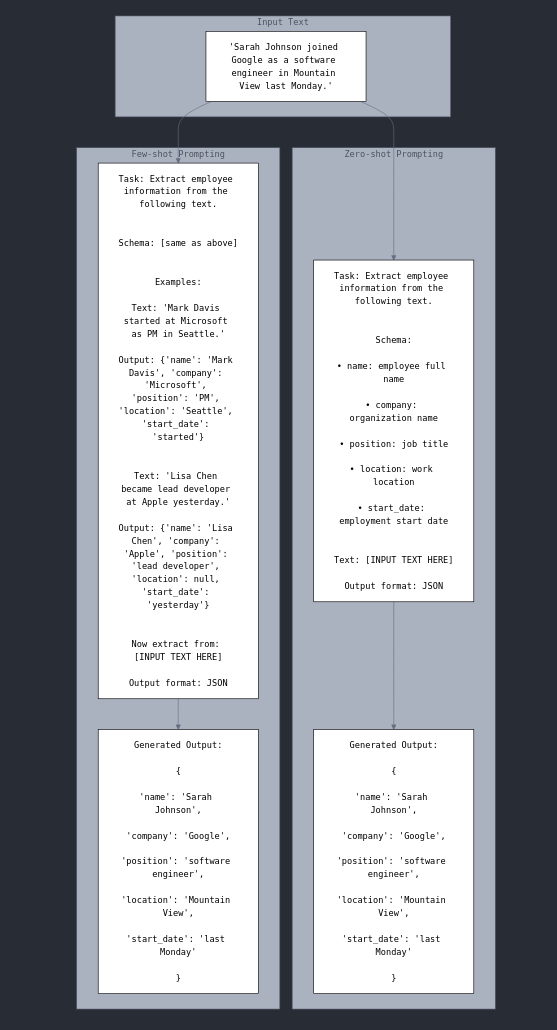
\includegraphics[width=0.8\linewidth]{images/zero_shot_vs_few_shot.png}
    \caption{Zero-shot vs Few-shot Prompting for Template Filling}
    \label{fig:placeholder}
\end{figure}

Schema-constrained prompting has also been investigated as a way to enforce output structure. Zhang et al.\ \cite{zhang2023sgptod} introduced SGP-TOD, where prompts embed schema definitions for task-oriented dialogue systems. By instructing the model to generate only values that fit the schema, they reduced invalid or inconsistent outputs. Practical systems follow the same idea: Google’s LangExtract \cite{google2024langextract} lets users define a JSON schema and then generates extractions that are automatically validated against it. While this approach provides consistency in output format, it remains monolithic and does not allow modular correction or multi-model validation.

Beyond hand-crafted design, some studies explore automated prompt optimization. Peng et al.\ \cite{peng2023check} propose a framework where candidate prompts are iteratively refined based on feedback signals, such as factual errors or schema mismatches. This “prompt tuning without training” approach suggests that prompts themselves can be systematically improved using evaluation signals, rather than relying only on human intuition.

In summary, prompt engineering has proven to be a powerful tool for adapting LLMs to information extraction tasks. It enables zero-shot and few-shot template filling, allows domain knowledge to be embedded into prompts, and supports schema-constrained generation. At the same time, it has clear limitations: prompts are often brittle, performance varies with phrasing, and external validation is still needed to ensure correctness. These weaknesses motivate research into more modular and interactive systems, where prompt design is combined with additional layers of control. The next subsection therefore examines multi-agent LLM systems, which distribute responsibilities across specialized agents to improve transparency, adaptability, and correction.


\subsection{Multi-Agent LLM Systems}
While single-model prompting can achieve strong results, it often struggles with reliability, transparency, and adaptability in complex tasks. Recent work has therefore explored multi-agent systems, where large language models are organized as a group of cooperating agents with different roles. Instead of relying on one model to handle everything, tasks such as extraction, validation, and correction can be split into smaller parts, each performed by a specialized agent.

\begin{figure}[hbt!]
    \centering
    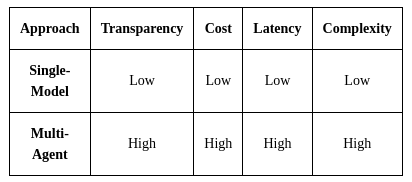
\includegraphics[width=0.5\linewidth]{images/single_vs_multi_model.png}
    \caption{Comparison of single-model and multi-agent approaches}
    \label{fig:placeholder}
\end{figure}

One of the best-known examples of this trend is HuggingGPT, introduced by Shen et al.\ \cite{shen2023hugginggpt}. In this framework, an LLM acts as a controller that delegates subtasks to external models hosted on the Hugging Face platform. The controller coordinates the results and integrates them into a final response. Liang et al.\ \cite{liang2023taskmatrix} proposed a similar system, TaskMatrix.AI, which connects LLMs with thousands of external APIs so that each subtask can be handled by the tool best suited for it. These studies show how LLMs can work as managers that coordinate specialized modules, rather than attempting to solve every step by themselves.

Other work has focused on applying multi-agent ideas directly to document and information extraction. Park et al.\ \cite{park2023generative} describe generative agents that cooperate to process documents: one agent extracts candidate entities, while another validates or reformats them according to schema constraints. This separation of roles reduces the cognitive load on any single model and makes the pipeline easier to debug, since errors can be traced back to a specific agent. Du et al.\ \cite{du2023improving} investigate multi-agent dialogue, where different agents simulate roles such as information seeker, verifier, and summarizer, in order to improve factual consistency. These ideas can be transferred to template filling, where one agent extracts fields, another checks them, and a third refines or corrects them.

Consensus-based multi-agent systems add another layer of reliability. Wu et al.\ \cite{wu2023autoagents} introduced AutoAgents, an open-source framework where multiple agents generate alternative outputs which are then compared, aggregated, or voted on. This ensemble-style approach reduces variance and improves robustness by leveraging diversity across agents. It mirrors classical redundancy methods but benefits from the contextual reasoning abilities of LLMs, making it especially useful in noisy or ambiguous input scenarios.

Despite their advantages, multi-agent systems face important challenges. They require more coordination and introduce overhead, since communication between agents can be costly and errors in one stage can still propagate. Designing reliable interfaces between agents is crucial, otherwise misalignments may cause cascading errors. In addition, evaluation of coordination quality is still underdeveloped; most benchmarks focus on the final output rather than the collaboration process itself. Finally, multi-agent pipelines often have longer latency and higher costs compared to single-model approaches.

In the context of this thesis, multi-agent systems are highly relevant because they address three requirements identified earlier: transparency, user correction, and adaptability. By splitting tasks into separate roles, they allow errors to be traced to specific stages (supporting transparency), corrections to be integrated incrementally, and domain knowledge to be embedded in specialized agents. At the same time, their higher cost and coordination complexity highlight trade-offs compared to simpler single-model systems. These trade-offs motivate the comparative evaluation carried out in this thesis, where multi-agent strategies are tested alongside monolithic and hybrid approaches.


\subsection{Evaluation of Requirements in Existing Solutions}
The reviewed approaches show steady progress in structured information extraction. Rule-based and statistical systems established transparent baselines but depended on handcrafted features and did not generalize well. Generative transformers (e.g., Du et al.\ \cite{du2021template}) enabled end-to-end template filling and improved accuracy. Speech-focused work (Sun et al.\ \cite{sun2023slot}) pushed extraction under noisy ASR inputs. Schema-centric methods and tools (Zhang et al.\ \cite{zhang2023sgptod}; Google LangExtract \cite{google2024langextract}) stabilized output formats, while constrained decoding \cite{anderson2017guided} enforced structure. Beyond extraction, Chen et al.\ \cite{le2025automated} showed schema-constrained generation for web testing. Multi-agent lines (Shen et al.\ \cite{shen2023hugginggpt}; Liang et al.\ \cite{liang2023taskmatrix}; Park et al.\ \cite{park2023generative}) introduced modularity, coordination, and validation. 

When judged against the requirements in the above Section, no single approach satisfies all of \textbf{R1--R6}. The consolidated table below summarizes what each work \emph{explicitly} supports (we mark a requirement as satisfied only if the paper/tool itself provides direct evidence; otherwise we mark ``---'' as \emph{not mentioned}).

% ===== Consolidated table (10 papers, R1--R6) =====
\begin{table*}[h!]
\centering
\renewcommand{\arraystretch}{1.25}
\setlength{\tabcolsep}{8pt}
\small
\begin{tabular}{|l|c|c|c|c|c|c|}
\hline
\textbf{Paper / Tool} & \textbf{R1} & \textbf{R2} & \textbf{R3} & \textbf{R4} & \textbf{R5} & \textbf{R6} \\
\hline
Du et al.\ 2021 \cite{du2021template} & \cmark & \cmark & \xmark & \xmark & \xmark & --- \\
Sun et al.\ 2023 \cite{sun2023slot} & \cmark & \cmark & \xmark & \xmark & \xmark & --- \\
Chen et al.\ 2025 \cite{le2025automated} & \cmark & \cmark & \xmark & \xmark & \xmark & --- \\
Google LangExtract 2024 \cite{google2024langextract} & \cmark & \cmark & \xmark & \xmark & \xmark & --- \\
Zhang et al.\ 2023 \cite{zhang2023sgptod} & \cmark & \cmark & \xmark & \xmark & \xmark & --- \\
Lin et al.\ 2021 \cite{lin2021leveraging} & \cmark & \cmark & \xmark & \xmark & \cmark & --- \\
Peng et al.\ 2023 \cite{peng2023check} & \cmark & \cmark & \xmark & \cmark & \cmark & --- \\
Shen et al.\ 2023 \cite{shen2023hugginggpt} & \cmark & \cmark & \cmark & \xmark & \cmark & --- \\
Liang et al.\ 2023 \cite{liang2023taskmatrix} & \cmark & \cmark & \xmark & \xmark & \cmark & --- \\
Park et al.\ 2023 \cite{park2023generative} & \cmark & \cmark & \cmark & \cmark & \cmark & --- \\
\hline
\end{tabular}
\caption{Consolidated evaluation of reviewed works against requirements R1--R6.}
\vspace{4pt}
\footnotesize \textit{Legend:} \cmark\,= satisfied; \xmark\,= not satisfied; ---\,= not mentioned.
\end{table*}


% ===== 2–3 lines per paper (brief evidence-based notes) =====
\paragraph{Du et al.\ 2021 \cite{du2021template}.}
End-to-end generative template filling outperforms pipelines on MUC-4 and models cross-event dependencies (R1, R2). No evidence spans, confidence scores, user correction, or adaptive learning are provided (R3--R5). Latency/usability not reported (R6).

\paragraph{Sun et al.\ 2023 \cite{sun2023slot}.}
Evaluates LLMs for slot filling from noisy ASR (SLURP), with prompt structures, LoRA, and LKI improving accuracy (R1, R2). No transparency or user-correction loop; adaptation is not defined as learning from corrections/ontologies (R3--R5). No latency reporting (R6).

\paragraph{Chen et al.\ 2025 \cite{le2025automated}.}
Combines screen transition/state graphs with LLMs to generate structured Selenium scripts (R1, R2). No interpretability, correction mechanisms, or adaptive learning (R3--R5). No runtime/latency analysis (R6).

\paragraph{Google LangExtract 2024 \cite{google2024langextract}.}
Production tool mapping text to user-defined JSON schemas with validation (R1, R2). Opaque single-model design with no interactive correction or learning from edits (R3--R5). No latency claims (R6).

\paragraph{Zhang et al.\ 2023 \cite{zhang2023sgptod}.}
Schema-guided prompting reduces invalid slot outputs in task-oriented dialogue (R1, R2). No span-level evidence, correction loop, or learning-from-corrections (R3--R5). No latency reporting (R6).

\paragraph{Lin et al.\ 2021 \cite{lin2021leveraging}.}
Slot descriptions enable zero-shot DST across unseen domains, supporting generalization (R1, R2, R5). Lacks transparency and user correction (R3, R4). No latency discussion (R6).

\paragraph{Peng et al.\ 2023 \cite{peng2023check}.}
Automated feedback improves factuality and structured outputs (R1, R2). Uses iterative prompt refinement as a correction signal and integrates external knowledge (R4, R5). No transparency or latency reporting (R3, R6).

\paragraph{Shen et al.\ 2023 \cite{shen2023hugginggpt}.}
LLM controller coordinates HF models; task planning and tool selection logs provide partial transparency (R1--R3). No explicit user-correction mechanism; adaptable via tool selection (R4, R5). No latency reporting (R6).

\paragraph{Liang et al.\ 2023 \cite{liang2023taskmatrix}.}
Connects LLMs with a large API ecosystem to perform varied tasks via structured calls (R1, R2); adaptable across domains (R5). No interpretability or correction loop (R3, R4). No latency metrics (R6).

\paragraph{Park et al.\ 2023 \cite{park2023generative}.}
Multi-agent document pipeline separates extraction and validation, improving traceability and enabling correction; modular agents support adaptation (R1--R5). No latency/usability characterization (R6).

% ===== Section wrap-up =====
\paragraph{Summary.}
Across R1--R6, current solutions contribute complementary strengths: end-to-end generative models lift accuracy; speech-focused methods add noise robustness; schema-guided designs stabilize formats; and multi-agent systems improve transparency, correction, and adaptability. Yet none meet all requirements simultaneously. This motivates the comparative experiments in later chapters, where we implement single-pass, iterative, consensus-based, and multi-agent designs and evaluate them with the same R1--R6 framework to quantify trade-offs in realistic, speech-driven scenarios.



\chapter{Concept}
This chapter presents the conceptual foundation of the proposed solution, grounded in the requirements and limitations identified in Chapter 2. The core objective is to transform unstructured narrative input—whether spoken or typed—into structured, schema-conformant templates through a modular, agent-based architecture. Unlike monolithic approaches that attempt end-to-end extraction in a single inference step, the proposed system decomposes the task into specialized subtasks, each handled by a dedicated agent with clearly defined responsibilities and interfaces.

The design is motivated by three critical shortcomings observed in existing work. First, single-model systems lack transparency: when extraction fails, it is difficult to trace whether the error originated in entity recognition, field mapping, or format normalization \cite{du2021template, sun2023slot}. Second, monolithic architectures are brittle under noisy or domain-specific input, as they cannot isolate and recover from localized failures \cite{wang2021spoken}. Third, current solutions provide limited support for iterative refinement, user correction, or learning from domain knowledge, restricting their adaptability in real-world deployments \cite{mialon2023augmented, park2023generative}.

The proposed Invox system addresses these limitations through a five-stage pipeline that enforces separation of concerns while preserving end-to-end coherence. Each agent operates on well-defined inputs and produces structured outputs that serve as inputs to downstream components. This modular design directly supports the six requirements established in Section 2.1: consistency is enforced through dedicated normalization (R1), extraction accuracy benefits from retrieval-augmented context (R2), intermediate artifacts enable traceability (R3), outputs remain editable at the end before final submission (R4), the system learns from historical templates and domain resources (R5), and architectural strategies can be selected to meet latency constraints (R6).

The remainder of this chapter is organized as follows. Section 3.1 derives the conceptual design from the analysis results, explaining how each requirement motivates specific architectural decisions. Section 3.2 describes the five modular agents that comprise the pipeline, detailing their individual responsibilities, inputs, outputs, and internal mechanisms. Section 3.3 presents four architectural strategies—Single-Pass Full Input, Iterative Single-Field Processing, Multi-LLM Consensus (Full), and Multi-LLM Consensus (Iterative)—that instantiate the same pipeline with different trade-offs in accuracy, latency, and cost. Section 3.4 provides the high-level system architecture and design, including context diagrams, container views, and process flows that illustrate how components interact in deployment scenarios. Detailed implementation and experimental validation are deferred to Chapters 4 and 5, respectively.

% \section{Concept Derivation from Analysis Results}
\label{sec:concept-derivation}

The conceptual design of the Invox system is derived systematically from the six requirements identified in Section~\ref{sec:requirements} and the gaps observed in existing approaches reviewed in Section~\ref{sec:related-work}. This section traces how each architectural decision directly addresses specific limitations in current template-filling systems, establishing the rationale for a modular, multi-agent design.

\subsection{From Monolithic to Modular Processing}
\label{subsec:monolithic-to-modular}

The analysis in Section~\ref{sec:related-work} revealed that monolithic approaches—where a single LLM performs extraction, normalization, and validation in one inference step—suffer from three fundamental weaknesses. First, they propagate errors across stages without providing mechanisms for localized recovery \cite{sun2023slot}. When entity recognition fails, subsequent field mapping inherits these errors, compounding inaccuracies. Second, they lack transparency: users cannot trace which part of the input led to which output, making error diagnosis difficult and undermining trust \cite{ribeiro2016should}. Third, they provide no intermediate points for user intervention, forcing corrections to be applied post-hoc rather than during processing \cite{amershi2019guidelines}.

These observations directly motivate the decomposition of the template-filling task into discrete, sequential stages. By separating transcription, retrieval, extraction, normalization, and verification into dedicated agents, the system gains three critical capabilities. Errors can be isolated to specific stages, allowing targeted debugging and recovery without reprocessing the entire pipeline. Intermediate outputs become visible and editable, supporting both transparency (R3) and user correction (R4). Finally, individual agents can be improved or replaced independently, enabling iterative refinement without destabilizing the overall architecture.

\subsection{Addressing Consistency Through Dedicated Normalization}
\label{subsec:consistency-normalization}

Requirement R1 demands that heterogeneous inputs—whether informal speech transcripts, chat messages, or multilingual notes—be transformed into uniform, comparable template entries. Existing generative systems often produce stylistically inconsistent outputs because the same model is responsible for both content extraction and format enforcement \cite{huang2024authorship}. This dual responsibility introduces variance: one inference may produce "08/16/2025" while another outputs "August 16, 2025" for the same date, even when guided by identical prompts.

The solution is to delegate normalization to a specialized Consistency Formatting (CF) agent that operates independently of extraction. Once the Information Extraction (IE) agent proposes candidate values, CF applies deterministic transformations—date standardization, entity canonicalization, and vocabulary alignment—ensuring that all outputs conform to predefined schemas. This separation ensures that extraction logic remains focused on identifying correct content, while formatting logic enforces structural and stylistic uniformity. The result is higher consistency across diverse inputs, directly satisfying R1.

\subsection{Retrieval-Augmented Generation for Domain Adaptation}
\label{subsec:rag-domain-adaptation}

Requirement R2 emphasizes robust information extraction under noisy, incomplete, and domain-specific conditions. Section~\ref{sec:related-work} showed that zero-shot LLMs struggle with specialized terminology, abbreviations, and implicit references common in industrial and healthcare contexts \cite{wang2021spoken}. While few-shot prompting improves performance, manually curating examples for every deployment scenario is impractical and does not scale across domains \cite{wei2022emergent}.

This motivates the introduction of a Retrieval-Augmented Generation (RAG) agent positioned between transcription and extraction. The RAG agent queries an indexed corpus of historical templates and domain glossaries, retrieving the $k$ most semantically similar examples for the current input. These examples are passed to the IE agent as dynamic few-shot context, grounding its reasoning in domain-specific patterns without requiring manual prompt engineering. This design directly supports R2 by improving extraction accuracy on specialized vocabulary, and also contributes to R5 (learning and adaptation) by leveraging organizational knowledge accumulated over time.

\subsection{Verification for Completeness and Cross-Field Consistency}
\label{subsec:verification-consistency}

Existing template-filling systems rarely validate their own outputs. Once fields are populated, the result is presented to the user without checking for missing required fields, contradictory values, or schema violations \cite{sun2023slot}. This places the entire verification burden on the user, increasing workload and reducing trust.

The Verification (VER) agent addresses this gap by performing three types of checks after normalization. Completeness checks ensure that all required fields have been populated or explicitly marked as unavailable. Cross-field consistency checks detect contradictions, such as an incident date that falls outside the reported shift time. Confidence scoring highlights uncertain extractions, directing user attention to fields most likely to require correction. When issues are detected, VER can trigger a clarification loop, prompting the user for additional input before re-applying CF and VER on the updated values. This design supports R3 (transparency) by making verification criteria explicit, and R4 (user correction) by enabling targeted intervention.

\subsection{Modularity as a Foundation for Flexibility}
\label{subsec:modularity-flexibility}

The evaluation in Section~\ref{subsec:limitations} demonstrated that no single existing system satisfies all six requirements simultaneously. Systems optimized for accuracy often sacrifice latency \cite{park2023generative}, while those prioritizing speed compromise on transparency or adaptability \cite{google2024langextract}. This trade-off is inherent to monolithic designs, where architectural choices are baked into a single model and cannot be adjusted post-deployment.

The modular pipeline enables flexible deployment strategies without changing the underlying components. The same five agents can be orchestrated in multiple ways: as a sequential single-pass system for low-latency scenarios, as an iterative slot-parallel architecture for higher accuracy, or as a multi-model consensus mechanism for critical applications where reliability outweighs cost. Section~\ref{sec:architectural-strategies} formalizes these strategies and analyzes their trade-offs. This flexibility directly addresses R6 (usability) by allowing latency constraints to guide strategy selection, while preserving modularity for future improvements.


This section summarizes how each architectural decision maps to the requirements established in Chapter~\ref{chap:analysis}. The modular design is not an arbitrary choice, but a direct consequence of the limitations observed in existing work and the operational constraints of real-world deployment contexts. The next section details the five agents that instantiate this design, specifying their inputs, outputs, and internal processing logic.
% \section{Five-Agent Architecture}
\label{sec:concept-architecture}

The modular architecture of \textit{Invox} is organized into five specialized agents. Each agent exposes a clear input/output contract, enabling component-level analysis, flexible substitution, and isolated improvement. This section characterizes the roles of the agents and their interconnections, independent of any particular deployment strategy.

\begin{figure}[H]
  \centering
  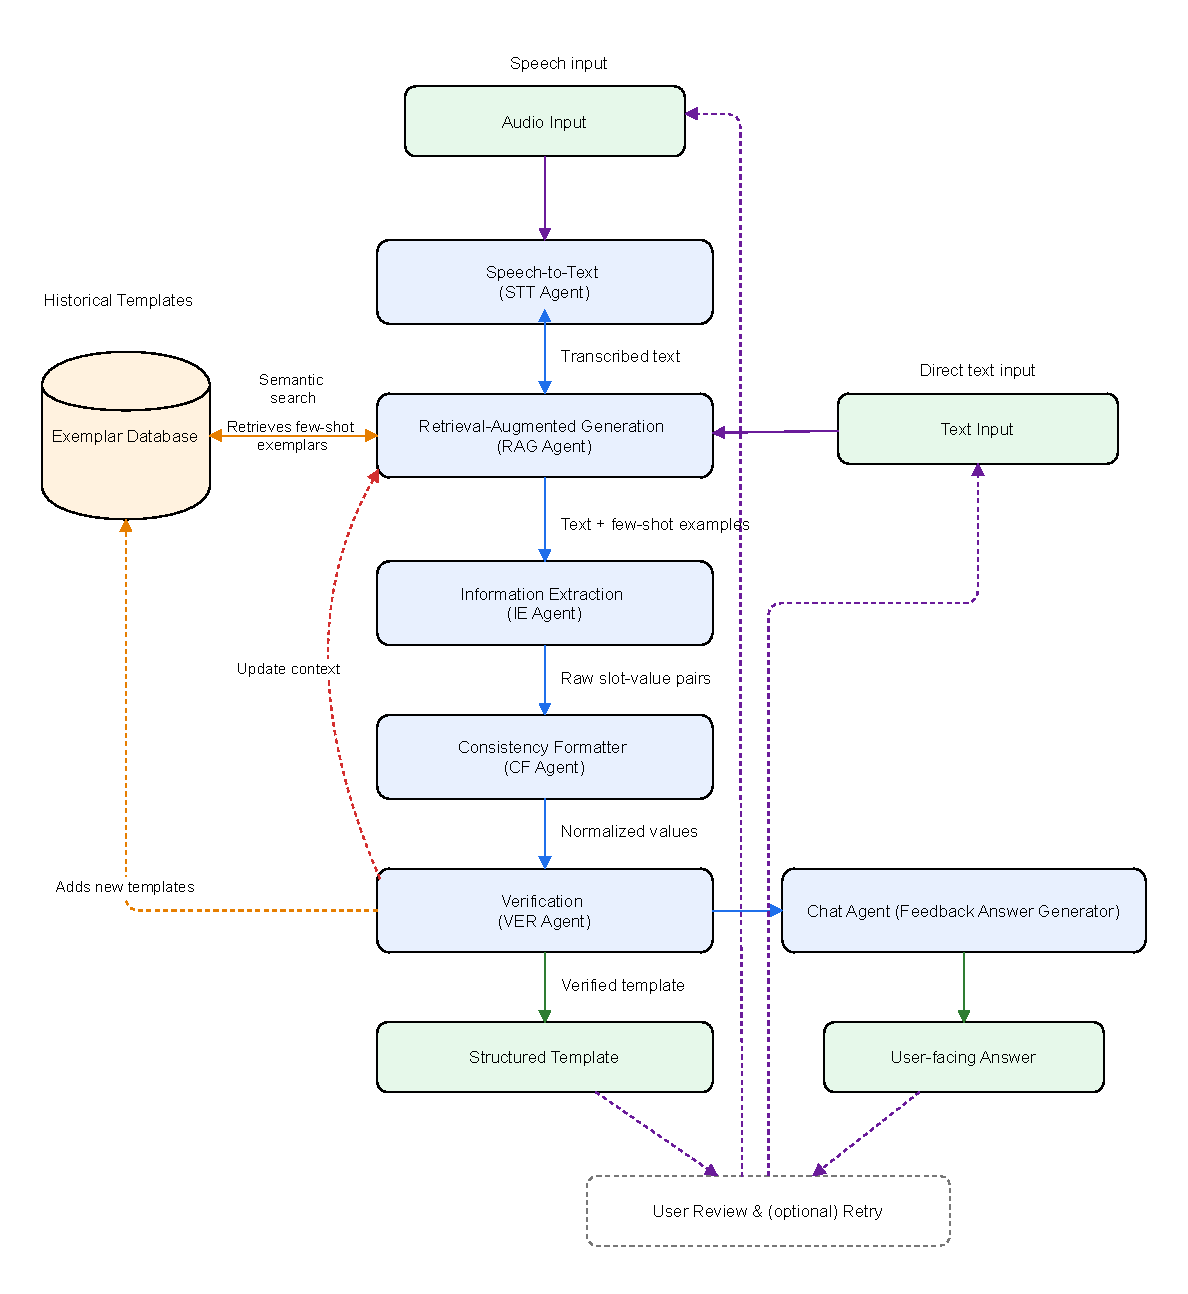
\includegraphics[width=1.0\linewidth]{images/agent_pipeline.drawio.pdf}
  \caption{Invox’s Five-Agent Pipeline}
  \label{fig:agent-pipeline}
\end{figure}



\subsection{Speech-to-Text Agent (STT)}
\label{subsec:stt-agent}

The STT agent converts spoken language into text using a Whisper-based transcription model \cite{radford2023whisper}. It accepts audio recordings as input and outputs transcribed text along with metadata such as word-level confidence scores, timestamps, and language detection results. As the focus of this work is the mapping from unstructured text to template fields, the STT component remains an adapter rather than the core of the architecture. Textual inputs bypass this stage and enter directly into the RAG agent.

\textbf{Design considerations.} The STT agent is deliberately shallow to maintain generality. Whisper was selected for its robustness to noise and multilingual support, which are critical in industrial environments where background machinery, accents, and code-switching are common \cite{fathullah2023prompting}. Alternative ASR systems could be substituted without affecting downstream components, provided they produce UTF-8 text output.

\subsection{Retrieval-Augmented Generation Agent (RAG)}
\label{subsec:rag-agent}

The RAG agent enhances extraction accuracy by retrieving relevant examples from historical data before template filling begins. It accepts the transcribed or typed text as input and queries an indexed corpus—comprising previously completed templates—using semantic similarity search over dense vector embeddings. The agent outputs the top-$k$ most relevant examples, which are passed alongside the user input to the IE agent as few-shot context.

\textbf{Retrieval mechanism.} The RAG agent encodes input text using a pretrained sentence transformer and performs cosine similarity search against stored template embeddings. The system returns $k$ ranked examples (typically $k = 3$–$5$), each containing the original text and its corresponding template completion.

\textbf{Design rationale.} This agent directly addresses R2 (information extraction) and R5 (learning and adaptation). By dynamically selecting examples tailored to the current input, the system avoids the brittleness of static few-shot prompts while benefiting from organizational memory \cite{mialon2023augmented}. The semantic search ensures that examples are retrieved based on conceptual similarity, making the system robust to paraphrasing and vocabulary variations. Over time, as more templates are completed and added to the index, extraction accuracy improves without requiring model retraining.

\subsection{Information Extraction Agent (IE)}
\label{subsec:ie-agent}

The IE agent performs the central task of transforming unstructured text into structured template fields. Its input consists of three components: (1) the free-form text (transcribed or provided directly), (2) the retrieved few-shot examples from the RAG agent, and (3) the target template schema specifying which fields need to be filled. The agent outputs candidate slot-value pairs for all specified fields in the template schema.

The agent operates by prompting a large language model with task-specific instructions and examples. For each field in the template schema, the model attempts to extract relevant information from the input text. If information for a particular field cannot be found in the text, the field is explicitly populated with a null value rather than being omitted. This ensures completeness while maintaining the structured output format.

\textbf{Processing approach:}
\begin{itemize}
    \item \textbf{Schema-driven extraction:} The agent processes all fields specified in the template schema, ensuring comprehensive coverage of the required information structure.
    \item \textbf{Evidence-based population:} Fields are populated only when supporting evidence is present in the input text, preventing hallucination of unsupported values.
    \item \textbf{Explicit null handling:} When information for a field is unavailable in the text, the field is explicitly marked as null, maintaining the complete output structure.
\end{itemize}

\textbf{Prompt structure.} The IE agent's prompt consists of four components: (1) task definition specifying the target schema and fields, (2) retrieved few-shot examples demonstrating successful extraction patterns, (3) the current user input text, and (4) output format constraints requiring JSON-structured responses that include all specified fields. This structure ensures consistent output formatting while leveraging the contextual understanding provided by few-shot examples \cite{zhang2023sgptod}.

\subsection{Consistency Formatting Agent (CF)}
\label{subsec:cf-agent}

The CF agent transforms the raw extracted values from the IE agent into standardized, schema-compliant formats. It accepts the slot-value pairs produced by the IE agent and applies deterministic normalization rules and schema validation to ensure consistency across all template outputs.

\textbf{Schema validation and normalization:}
\begin{itemize}
    \item \textbf{Data type enforcement:} Converts extracted values to appropriate data types (dates to ISO format, numbers to numerical types, etc.) and validates against schema constraints
    \item \textbf{Value canonicalization:} Standardizes variations using deterministic rules (e.g., ``Sept. 11'' → ``2001-09-11'', ``USA'' → ``United States'')
    \item \textbf{Controlled vocabulary mapping:} Enforces domain-specific conventions by mapping extracted terms to predefined categories for incident types, equipment codes, and other standardized fields
    \item \textbf{Schema compliance checking:} Validates that all values conform to the template schema requirements, including format constraints and value ranges
\end{itemize}

\textbf{Normalization approach.} The CF agent employs both deterministic transformations and LLM-based resolution for ambiguous cases. Structured data types like dates, numbers, and standard identifiers are normalized using regular expressions and parsing libraries. For ambiguous entities—such as informal location names or context-dependent equipment codes—the agent can prompt an LLM with the original context and domain glossaries to resolve variations. This hybrid approach balances precision with contextual awareness while maintaining deterministic behavior for well-defined formats.

\textbf{Design rationale.} By separating normalization from extraction, the system ensures consistent output formatting regardless of input variations while enforcing schema compliance. This addresses requirement R1 (consistency) and allows the IE agent to focus solely on content identification rather than format enforcement \cite{gatt2018survey}. The CF agent also reduces evaluation noise by ensuring that performance comparisons across different extraction strategies are not confounded by formatting inconsistencies.

\subsection{Verification Agent (VER)}
\label{subsec:ver-agent}

The VER agent performs comprehensive quality assessment on the structured template produced by the CF agent. It accepts the normalized slot-value pairs as input and generates a fully verified template with confidence scoring, field-level annotations, and interactive clarification capabilities.

\textbf{Quality assessment components:}
\begin{itemize}
    \item \textbf{Confidence scoring:} Assigns confidence scores to each populated field based on extraction quality, evidence strength, and internal consistency metrics
    \item \textbf{Field annotations:} Provides detailed annotations for each field indicating the source evidence, extraction method, and any processing notes
    \item \textbf{Conflict detection:} Identifies internal contradictions or inconsistencies between related fields (e.g., conflicting dates, incompatible equipment types)
    \item \textbf{Completeness validation:} Flags required fields that remain empty or contain insufficient information
\end{itemize}

\textbf{Interactive clarification system.} When low-confidence fields, conflicts, or missing required information are detected, the VER agent generates targeted chat messages to solicit user clarification. These messages are context-aware and focus specifically on the uncertain aspects of the template, enabling iterative refinement through user feedback. The system maintains conversation history to provide context for subsequent clarification rounds.

\textbf{Final output generation.} The VER agent produces the completed template with all quality annotations, making transparent which fields are highly reliable versus those requiring user verification. This includes:
\begin{itemize}
    \item Confidence scores for automated quality assessment
    \item Evidence references linking extracted values to source text spans
    \item Clear indicators of fields that may need user attention
    \item Structured data ready for database integration or further processing
\end{itemize}

\textbf{Design rationale.} VER directly supports R3 (transparency) by providing comprehensive field-level annotations and confidence metrics, and R4 (user correction) through its interactive clarification system. By centralizing quality assessment and user interaction in a dedicated agent, the system ensures consistent verification standards while maintaining clear separation from the extraction and normalization processes \cite{park2023generative}.

\subsection{Agent Interfaces and Data Flow}
\label{subsec:agent-interfaces}

Table~\ref{tab:agent-interfaces} summarizes the interface of each agent. By separating their responsibilities and outputs, the architecture supports substitution of different models, logging of intermediate states, and detailed error analysis. Figure~\ref{fig:agent-pipeline-enhanced} illustrates the sequential data flow through the five agents for both audio and text inputs.

\begin{table}[h]
\centering
\begin{tabular}{p{2.5cm}p{5cm}p{5.5cm}}
\toprule
\textbf{Agent} & \textbf{Input} & \textbf{Output} \\
\midrule
\textbf{STT} & Audio signal & Transcribed text with metadata (confidence scores, timestamps) \\
\midrule
\textbf{RAG} & Text (transcribed or direct input) & Top-$k$ retrieved examples with relevance scores and template mappings \\
\midrule
\textbf{IE} & Text + retrieved examples + template schema & Candidate slot-value pairs (null for unavailable fields) \\
\midrule
\textbf{CF} & Raw slot-value pairs & Normalized values with schema validation and format standardization \\
\midrule
\textbf{VER} & Normalized slot-value pairs & Verified template with confidence scores, field annotations, and clarification prompts \\
\bottomrule
\end{tabular}
\caption{Invox's Agent interfaces and data flow}
\label{tab:agent-interfaces}
\end{table}

The next section formalizes four deployment strategies that instantiate this architecture with different orchestration patterns, trading off accuracy, latency, and computational cost.


% \section{Architectural Strategies}
\label{sec:architectural-strategies}

While the modular five-agent pipeline defines the general structure of the \textit{Invox} system, its effectiveness depends on how large language models (LLMs) are deployed within the \textit{Information Extraction} and \textit{Verification} stages. Different architectural strategies offer distinct trade-offs in terms of accuracy, robustness, latency, cost, and transparency. This section outlines four strategies and illustrates them using a common example to enable direct comparison.

For all examples, we use the following input derived from the MUC-4 benchmark:  
\textit{``On March 3, 1992, in Bogotá, a powerful car bomb exploded outside the Ministry of Defense, damaging nearby buildings and injuring 25 people, though no fatalities were reported. Authorities suspect a left-wing guerrilla group, but responsibility remains unconfirmed.''}

This example introduces multiple attributes (date, location, event type, casualties, suspected perpetrators, and epistemic uncertainty), allowing us to highlight the strengths and weaknesses of each strategy under realistic conditions.

\subsection{Strategy S1: Single-Pass (Full-Input, Single-LLM)}
\label{subsec:strategy-s1}

\textbf{Overview.}  
In the simplest approach, a single LLM receives the complete transcript—along with few-shot examples retrieved by the RAG agent—and directly generates all template fields in one inference pass. The extracted values then proceed through Consistency Formatting (CF) and Verification (VER) before finalization.

\begin{figure}[H]
  \centering
  \includegraphics[width=1.0\linewidth]{images/single-llm-full-input.drawio.pdf}
  \caption{Strategy: Full-Input, Single-LLM}
  \label{fig:single-llm-full-input}
\end{figure}

\textbf{Advantages.}  
This strategy is computationally efficient, requiring only one IE model call. It minimizes latency and API costs, making it suitable for high-throughput scenarios. The inclusion of RAG-retrieved examples improves domain adaptation compared to zero-shot prompting, while CF and VER stages provide downstream quality assurance.

\textbf{Limitations.}  
If the LLM misinterprets a critical ambiguity—such as treating ``suspected guerrilla group'' as a confirmed perpetrator—the error propagates through CF (which normalizes the incorrect value) and may only be flagged by VER if confidence thresholds are exceeded. The single inference point offers no redundancy, making the system vulnerable to model-specific biases or hallucinations \cite{du2020event}.

\subsection{Strategy S2: Iterative (Slot-wise, Single-LLM)}
\label{subsec:strategy-s2}

\textbf{Overview.}  
Each template slot is extracted by an independent LLM call with a slot-specific prompt. Slots can be processed sequentially or in parallel. The RAG agent retrieves relevant examples once at the beginning, and these are included in every slot-level prompt. Results are then passed to CF and VER for normalization and validation.

\begin{figure}[H]
  \centering
  \includegraphics[width=1.0\linewidth]{images/single-llm-slot-wise.drawio.pdf}
  \caption{Strategy: Slot-wise, Single-LLM}
  \label{fig:single-llm-slot-wise}
\end{figure}

\textbf{Advantages.}  
Slot independence isolates errors: if the perpetrator field is uncertain, only that slot requires re-extraction. This improves transparency (R3) by making it clear which fields are problematic. Parallelization across slots can reduce wall-clock latency on multi-core systems, though total computational cost increases. The strategy also supports slot-specific prompt engineering, allowing prompts to be tuned for date extraction, entity recognition, or casualty parsing independently.

\textbf{Limitations.}  
The approach increases inference cost linearly with the number of slots. For templates with 15–20 fields, this becomes expensive. Additionally, slot-level prompts lack cross-field context: the model extracting casualties does not see the perpetrator information, which may reduce coherence in cases where fields are interdependent \cite{sun2023slot}.

\subsection{Strategy S3: Multi-LLM Consensus (Full-Input)}
\label{subsec:strategy-s3}

\textbf{Overview.}  
Multiple LLMs—either different models (e.g., GPT-4, Claude, DeepSeek) or multiple runs of the same model with varied prompts—each generate a complete template from the full transcript and RAG-retrieved examples. Their outputs are compared by the Internal Verifier which has results from multiple llms, text input and the RAG examples, which selects the most consistent or reliable values using consensus rules such as majority voting or confidence-weighted aggregation.

\begin{figure}[H]
  \centering
  \includegraphics[width=1.0\linewidth]{images/multiple-llm-full-input.drawio.pdf}
  \caption{Strategy: Full-Input, Multiple-LLM}
  \label{fig:multiple-llm-full-input}
\end{figure}

\textbf{Advantages.}  
Ensemble diversity reduces systematic bias: if one model hallucinates or misinterprets ambiguous phrasing, others may produce more faithful outputs. Consensus mechanisms increase robustness, particularly when models disagree on uncertain fields. This strategy also preserves cross-field context, as each model sees the full input during extraction \cite{wu2023autoagents, park2023generative}.

\textbf{Limitations.}  
Computational cost increases linearly with the number of models. If all models converge on the same misinterpretation—due to shared training biases or ambiguous input phrasing—consensus provides no advantage. The strategy also requires careful tuning of aggregation rules: simple majority voting may discard nuanced or hedged outputs (e.g., "suspected") in favor of overly confident but incorrect answers.

\subsection{Strategy S4: Multi-LLM Consensus (Slot-wise)}
\label{subsec:strategy-s4}

\textbf{Overview.}  
Each slot is extracted independently by multiple LLMs, and consensus is reached per field before aggregating results. This combines the granularity of S2 (slot-wise processing) with the robustness of S3 (multi-model consensus). Their outputs are compared by the Internal Verifier which has results from multiple llms, text input and the RAG examples, which selects the most consistent or reliable values using consensus rules such as majority voting or confidence-weighted aggregation. Results are then passed through CF and VER. 

\begin{figure}[H]
  \centering
  \includegraphics[width=1.0\linewidth]{images/multiple-llm-slot-wise.drawio.pdf}
  \caption{Strategy: Slot-wise, Multiple-LLM}
  \label{fig:multiple-llm-slot-wise}
\end{figure}

\textbf{Advantages.}  
This strategy offers the highest reliability by applying ensemble methods at the most granular level. Slot-level consensus allows diverse models to specialize: one model may excel at date parsing, another at casualty extraction. Error isolation remains strong, as each field is independently verified. The approach is well-suited for safety-critical domains where accuracy justifies cost.

\textbf{Limitations.}  
Computational cost scales as (number of slots) × (number of models), making this the most expensive strategy. For a 15-field template with 3 models, this requires 45 LLM calls per document. Latency increases unless aggressive parallelization is employed. Additionally, consensus logic becomes more complex when models produce semantically equivalent but syntactically different outputs (e.g., "25 injured" vs. "25 people hurt"), requiring robust normalization before voting.

\subsection{Summary and Trade-Off Analysis}
\label{subsec:strategy-summary}

These four strategies represent different points in the trade-off space between accuracy, robustness, latency, and cost. Table~\ref{tab:strategy-comparison} summarizes their characteristics.

\begin{table}[H]
\centering
\begin{tabular}{lccccc}
\toprule
\textbf{Strategy} & \textbf{LLM Calls} & \textbf{Error Isolation} & \textbf{Robustness} & \textbf{Latency} & \textbf{Cost} \\
\midrule
S1: Single-Pass & 1 & L & L & L & L \\
S2: Iterative & $n$ (slots) & H & M & M & M \\
S3: Consensus (Full) & $m$ (models) & L & H & M & H \\
S4: Consensus (Slot) & $n \times m$ & H & H & H & H \\
\bottomrule
\end{tabular}
\caption{Comparison of architectural strategies. $n$ = number of slots, $m$ = number of models. L=Low, M=Medium, H=High.}
\label{tab:strategy-comparison}
\end{table}

\textbf{Selection criteria.} Strategy choice depends on deployment constraints:
\begin{itemize}
    \item \textbf{S1} is suitable for high-throughput applications where speed and cost matter more than perfect accuracy.
    \item \textbf{S2} enables fine-grained debugging and is appropriate when specific fields are known to be problematic.
    \item \textbf{S3} balances robustness and context preservation, making it suitable for general-purpose deployments.
    \item \textbf{S4} provides maximum reliability for critical applications where errors have serious consequences (e.g., medical records, regulatory reporting).
\end{itemize}

Chapter 5 empirically evaluates these strategies on the MUC-4 benchmark, also quantifying their performance across the six requirements (R1–R6) established in Chapter 2.\begin{figure}
    \centering
    \includegraphics[width=0.5\linewidth]{sa.png}
    \caption{Enter Caption}
    \label{fig:placeholder}
\end{figure}

\section{System Architecture and Design}
\label{sec:concept-design}

This section presents the high-level architecture of the Invox system using the C4 model, which structures architectural documentation into hierarchical levels: context (system boundaries and external actors), containers (major components and their interactions), and process (dynamic execution flow). These views provide a comprehensive understanding of how the conceptual design translates into a deployable architecture.

\subsection{Context View: System Boundaries and External Actors}
\label{subsec:context-view}

\begin{figure}[H]
  \centering
  \includegraphics[width=1\linewidth]{images/c4_context.drawio.pdf}
  \caption{Context diagram showing system boundaries and external actors.}
  \label{fig:c4-context}
\end{figure}

The context diagram (Figure~\ref{fig:c4-context}) positions Invox within its operational environment. The system interacts with three categories of external actors:

\textbf{Primary users} are domain experts—such as factory operators, medical staff, or administrative personnel—who provide unstructured input (speech or text) and review populated templates. They interact with the system through a web-based interface or mobile application.

\textbf{Data sources} include historical template repositories, domain-specific glossaries, and organizational knowledge bases. These are accessed by the RAG agent to retrieve contextually relevant examples. In regulated environments, these repositories may reside behind secure access controls.

\textbf{External services} consist of third-party APIs for LLM inference (OpenAI GPT-4, Anthropic Claude, DeepSeek), speech recognition (OpenAI Whisper), and search infrastructure (OpenSearch). The system communicates with these services over REST APIs.

\subsection{Container View: Internal Component Structure}
\label{subsec:container-view}

The container diagram (Figure~\ref{fig:c4-container}) decomposes Invox into its major internal components and clarifies how requests flow through the system.

\textbf{Client access.} Users interact with the system via the \emph{API Gateway}, which supports HTTP, HTTPS, or tRPC protocols. This is the only entry point for structured input requests. For raw audio, users may also call the \emph{STT Service} directly to obtain transcribed text.

\textbf{STT Service.} The STT service wraps the Whisper model, invokes the external ASR provider, and returns transcribed text enriched with metadata such as confidence scores, timestamps, and language detection. Transcribed text is returned to the client for display or routed back into the pipeline.

\textbf{RAG Service.} Once the API Gateway accepts a request, it forwards it into the backend pipeline starting with the RAG service. This service embeds the input, queries the \emph{Vector Index}, and enriches the request with semantically relevant examples.

\textbf{IE Service.} Using the enriched context, the IE service constructs prompts and invokes the configured LLM providers. Depending on the strategy (S1–S4), this may involve a single call, slot-wise calls, or multiple model invocations. Results are returned as candidate slot-value pairs.

\textbf{CF Service.} The CF service normalizes the extracted values (e.g., dates, entities) and enforces schema constraints to produce a consistent intermediate template.

\textbf{VER Service.} 
The verification service ensures completeness, consistency, and confidence of the template. It assigns confidence scores, detects conflicts, flags missing fields, and can trigger clarification requests via the API Gateway. Finalized templates, enriched with quality metadata, are stored in both the \emph{Template Repository} and the \emph{Vector Index}. This service is internal-only and not directly accessible to clients.

\textbf{Data stores.} 
\begin{itemize}
  \item \emph{Template Repository} stores finalized templates for future retrieval.
  \item \emph{Vector Index} holds dense embeddings for retrieval-augmented generation.
\end{itemize}

\textbf{End-to-end flow.} After verification, the finalized template is stored, indexed, and routed back through the API Gateway to the client as the official response.

\begin{figure}[H]
  \centering
  \includegraphics[width=1\linewidth]{images/c4_container.drawio.pdf}
  \caption{Corrected container diagram showing request flow through internal components and external dependencies.}
  \label{fig:c4-container}
\end{figure}

\subsection{Process View: Workflow and Decision Logic}
\label{subsec:process-view}

The process diagram (Figure~\ref{fig:bpmn}) presents the dynamic execution flow. The workflow follows this structure:

\textbf{Input reception.} User submits audio or text. Audio is processed by the STT service; text requests proceed via the API Gateway into the backend pipeline.

\textbf{Retrieval.} The RAG service queries the vector index and returns top-$k$ examples. If retrieval fails, the system falls back to zero-shot prompting.

\textbf{Extraction.} The IE service invokes the LLM(s) according to the chosen strategy. For multi-model strategies, all responses are collected before proceeding.

\textbf{Formatting.} CF normalizes extracted values and enforces schema constraints, flagging any that cannot be normalized for manual review.

\textbf{Verification.} VER checks consistency, completeness, and confidence. Possible outcomes are: (1) Pass—template is complete and returned; (2) Clarification required—system prompts user and re-executes IE $\rightarrow$ CF $\rightarrow$ VER; (3) Low confidence—template returned with uncertain fields for user review.

\textbf{Finalization.} Verified templates are stored in the repository, indexed for future retrieval, and returned to the client. Users may still edit fields before final submission.

\begin{figure}[H]
  \centering
  \includegraphics[width=1.0\linewidth]{images/bpmn_process_flow.pdf}
  \caption{Process diagram showing workflow and decision logic.}
  \label{fig:bpmn}
\end{figure}


\chapter{Implementation}
The conceptual architecture introduced in the previous chapter provides the theoretical foundation for transforming unstructured speech into structured templates. This chapter shifts focus from design to realization, demonstrating how the multi-agent pipeline was implemented in practice. The implementation details cover technology selection, system workflow, concrete agent implementations, and the realization of the four architectural strategies. Finally, challenges and key design decisions encountered during development are discussed.

\section{Technology Stack and Rationale}
\label{sec:tech-stack}

The implementation of the \textit{Invox} system employs a modular monolith architecture that balances development simplicity with operational flexibility. The core application executes as a single Node.js service containing all five agents, while specialized components such as vector search and embedding generation operate as external services. This hybrid approach preserves the benefits of modular design while avoiding the operational complexity typically associated with fully distributed microservice deployments \cite{fowler2015monolith,microservices_newman}.

\subsection*{Architecture Pattern: Modular Monolith with External Services}

The system follows a modular monolith pattern in which all agents (STT, RAG, IE, CF, VER) are implemented as cohesive modules within a single Node.js application. This design choice offers several advantages: a unified codebase that reduces coordination overhead, simplified debugging, and consistent versioning across agents. In-process inter-agent communication minimizes latency compared to network-based microservices, while modularity is maintained through well-defined interfaces that preserve separation of concerns.

External specialized services are integrated via network calls. \textbf{OpenSearch} provides vector similarity search, accessible through \texttt{http://opensearch:9200}; a dedicated embedding service generates dense vector representations; and external LLM APIs (OpenAI, Google) handle model inference. This hybrid approach leverages specialized infrastructure where necessary, while retaining the core template-filling logic within a unified application \cite{opensearch_knn}.

\subsection*{Containerization and Deployment}

The entire system is containerized using \textbf{Docker}. The main application runs in a single container, ensuring a consistent runtime environment across development and production. Containerization simplifies dependency management, enables horizontal scaling through replication, and facilitates seamless integration with external services. \textbf{Docker Compose} orchestrates the multi-service deployment, coordinating the main application container alongside OpenSearch and other dependencies \cite{docker_docs}.

\subsection*{Backend Implementation}

The backend is implemented in \textbf{Node.js} with \textbf{Express}, providing a robust foundation for the agent pipeline. The system employs the \textbf{Vercel AI SDK} to realize a plugin-like architecture for LLM integration. This abstraction enables seamless switching between AI providers (OpenAI, Google, Anthropic), simplifies the addition of new models with minimal code changes, and future-proofs the system against the rapid evolution of the AI ecosystem \cite{llm_orchestration_survey}. Type-safe communication between frontend and backend is achieved through \textbf{tRPC}, while \textbf{JSON} serves as a flexible exchange format for inter-agent communication.

\subsection*{External Service Integration}

\textbf{OpenSearch} functions as the vector database for the RAG agent, enabling efficient semantic search over historical templates. A dedicated embedding generation service produces dense vector representations, which underpin similarity matching. Both services expose \textbf{REST APIs}, maintaining clear service boundaries while enabling specialized functionality \cite{opensearch_knn}.

\subsection*{Frontend Interface}

The user interface is implemented in \textbf{React}, selected for its component-based architecture that aligns naturally with the modular design of the template-filling system. React's virtual DOM and state management capabilities enable efficient rendering of dynamic content, such as structured templates and extracted fields with confidence indicators.

To ensure modern and accessible UI design, the system integrates the \textbf{shadcn/ui} component library. This provides reusable, consistent components with built-in design principles, thereby reducing frontend development overhead while ensuring a professional user experience for template review and correction workflows.

\subsection*{Data Persistence and Retrieval}

Persistent storage is provided by \textbf{PostgreSQL}, a relational database well-suited for structured data with complex relationships. The MUC-4 template schema maps naturally onto relational structures: fields such as incident type, date, and location are represented as structured columns, while more flexible attributes are stored in \texttt{JSONB} to allow schema evolution \cite{postgresql_jsonb}.

The \textbf{Sequelize} ORM is employed for schema definition, object mapping, secure query generation, and migration management. For vector similarity search, \textbf{OpenSearch} with the \texttt{knn} plugin enables efficient retrieval of relevant historical templates using dense embeddings \cite{opensearch_knn}.

\subsection*{Authentication and Security}

Authentication and role-based access control are managed via \textbf{Keycloak}, an open-source identity and access management solution supporting OAuth2 and OpenID Connect \cite{rfc6749,openid_connect}. Keycloak ensures secure integration with backend services and allows fine-grained role assignments—essential for collaborative workflows in which different users require distinct levels of access to system functionality.

\subsection*{Architecture Rationale}

The modular monolith pattern was chosen as a pragmatic balance between simplicity and flexibility. It combines the development velocity of a monolith with the architectural clarity of modular design \cite{fowler2015monolith}. The plugin-oriented LLM integration enabled by the Vercel AI SDK ensures adaptability to new models and capabilities as the field evolves, while containerized deployment guarantees reliable operation at scale. This architecture thereby provides a future-proof, maintainable, and efficient foundation for the \textit{Invox} system.

\section{System Workflow}
\label{sec:system-workflow}

This section describes the operational workflow of the Invox system, tracing the transformation of unstructured input into verified structured templates. The workflow implements the conceptual pipeline from Chapter~\ref{chap:concept} through a sequence of processing stages with user-driven quality control.

\subsection*{End-to-End Processing Flow}

The system workflow begins with user input and proceeds through six sequential stages:

\begin{enumerate}
    \item \textbf{Input Reception}: Users provide input through speech (audio recording) or direct text entry via the web interface. The system accepts both modalities and routes them appropriately through the processing pipeline.
    
    \item \textbf{Speech Recognition}: For audio inputs, the system invokes the Whisper ASR service to generate transcripts with confidence scores and timestamps. Text inputs proceed directly to the next stage.
    
    \item \textbf{Context Retrieval}: The RAG agent queries the vector database to retrieve the most relevant historical templates and examples, providing contextual guidance for the extraction process.
    
    \item \textbf{Information Extraction}: Based on the selected strategy (S1–S4), the system processes the input:
    \begin{itemize}
        \item \textbf{S1 (Single LLM)}: A single language model extracts all template fields in one pass
        \item \textbf{S2 (Slot-wise)}: Multiple LLM calls extract each field independently  
        \item \textbf{S3/S4 (Multi-LLM)}: Multiple models generate candidate answers, with a dedicated judge LLM selecting the optimal response through comparative analysis
    \end{itemize}
    
    \item \textbf{Consistency Enforcement}: The CF agent normalizes dates to ISO format, standardizes entity names, and enforces schema compliance through deterministic transformation rules.
    
    \item \textbf{Quality Assessment and Presentation}: The system assigns confidence scores to each extracted field and presents the complete template to the user for review and potential correction.
\end{enumerate}

\subsection*{User-Driven Quality Control}

The system employs a user-in-the-loop approach where quality assurance is primarily driven by human judgment:

\textbf{Confidence-Based Presentation}: Fields with lower confidence scores are visually highlighted, directing user attention to potentially problematic extractions.

\textbf{Multi-Model Decision Making}: In strategies S3 and S4, the judge LLM evaluates candidate answers from multiple models, selecting the most appropriate response based on coherence, accuracy, and alignment with the input context.

\textbf{User-Initiated Reprocessing}: If users are unsatisfied with results, they can modify their input and resubmit for reprocessing, creating an iterative refinement cycle driven by human assessment rather than automated detection.

\subsection*{Knowledge Accumulation}

Successfully processed templates are indexed in the vector database, enabling the RAG agent to leverage an expanding knowledge base for improved context retrieval in future processing cycles.
\section{Agent Implementation}
\label{sec:impl-agents}

This section details the concrete implementation of each agent in the Invox system, covering their API contracts, processing logic, and integration patterns. Each agent exposes well-defined TypeScript interfaces and follows consistent error handling patterns. The implementation is designed to be domain-agnostic, supporting arbitrary template schemas across healthcare, manufacturing, administrative, and other domains.

\subsection{Speech-to-Text (STT) Agent}
\label{subsec:impl-stt}

The STT agent provides a single entry point \texttt{transcribeForm} that converts audio inputs to structured transcripts using OpenAI's Whisper model.

\textbf{API Contract:}
\begin{verbatim}
interface TranscribeInput {
  file: {
    base64: string;         // Base64-encoded audio data
    mimetype: string;       // "audio/wav" | "audio/mpeg" | "audio/m4a"
    originalname: string;
  };
}

interface TranscribeResponse {
  transcript: string;           // Full transcribed text
  language: string;             // Detected language code (ISO 639-1)
  durationInSeconds: number;    // Audio duration
  segments?: Array<{            // Optional word-level timing
    start: number;
    end: number;
    text: string;
    confidence?: number;
  }>;
}
\end{verbatim}

\textbf{Implementation:} The agent decodes Base64 audio data into buffers and invokes the Whisper API via the Vercel AI SDK. Long audio files (>25MB or >10 minutes) are automatically chunked with 10\% overlap to ensure context preservation at boundaries. The agent returns word-level timestamps and confidence scores when available, enabling downstream agents to trace extracted values back to specific audio segments. Failed transcriptions (e.g., due to excessive noise or unsupported formats) throw structured errors that the orchestrator can handle gracefully, either by requesting re-recording or falling back to manual text entry.

\textbf{Configuration:} Temperature is set to 0 for deterministic output. Language detection is automatic unless overridden by the client. Voice activity detection (VAD) filters out silence and non-speech segments to improve accuracy.
\subsection{Retrieval-Augmented Generation (RAG) Agent}
\label{subsec:impl-rag}

The RAG agent implements semantic search over historical templates through the \texttt{getFewShotsFromTranscript} function, which retrieves contextually relevant examples to guide the information extraction process.

\textbf{API Contract:}
\begin{verbatim}
interface RAGInput {
  transcript: string;           // Input text for similarity search
  fields: FormTemplateField[];  // Target schema for field mapping
  k?: number;                   // Number of examples (default: 5, max: 5)
}

interface FewShot {
  text: string;                 // Truncated historical transcript
  expected: Record<string, {    // Field ID → normalized value
    value: unknown | null;
    evidence?: { transcriptSnippet?: string };
  }>;
}
\end{verbatim}

\textbf{Implementation:} The agent generates dense vector embeddings using OpenAI's \texttt{text-embedding-3-large} model. A key implementation detail is the embedding generation process: the input text is prefixed with \texttt{templateId=\${TEMPLATE\_ID}} to create template-aware embeddings that improve retrieval relevance within specific template contexts.

The agent performs k-nearest neighbor search using cosine similarity in OpenSearch with the \texttt{knn\_score} script. The search query filters results by template ID to ensure schema compatibility and uses a \texttt{script\_score} approach for efficient vector similarity computation.


\textbf{Result Processing:} Retrieved documents undergo post-processing where transcript texts are truncated to a maximum character limit (default: 1200 characters) to maintain prompt efficiency. The \texttt{toExpectedShape} function maps raw database results to the expected field schema, ensuring that only fields present in the current template schema are included in the output.

\textbf{Error Handling:} The implementation includes robust error handling for embedding generation failures and OpenSearch connectivity issues. If retrieval fails, the system gracefully falls back to zero-shot extraction, ensuring continuous operation despite temporary infrastructure problems.


\subsection{Information Extraction (IE) Agent}
\label{subsec:impl-ie}

The IE agent implements four extraction strategies through unified functions corresponding to S1–S4. All strategies share a common preprocessing pipeline and differ only in their orchestration of LLM calls.

\textbf{API Contract:}
\begin{verbatim}
interface IEInput {
  oldTranscript?: string;       // Previous context (for incremental updates)
  newTranscript: string;        // New user input (primary extraction source)
  fields: FormTemplateField[];  // Schema definition
  currentValues?: Record<string, CurrentFieldValue>;
  strategy: "S1" | "S2" | "S3" | "S4";
  fewShots?: RAGOutput['examples'];  // Retrieved examples from RAG
  locale?: string;              // e.g., "en-US", "de-DE"
  timezone?: string;            // e.g., "Europe/Berlin", "America/New_York"
  templateId?: string;          // For logging and monitoring
}

interface CurrentFieldValue {
  value: any;
  locked?: boolean;             // If true, field is never overwritten
  source?: "ai" | "manual";     // Origin of current value
}

interface IEOutput {
  filled: Record<string, FilledField>;
  model: string;                // Model identifier(s) used
  confidence?: Record<string, number>;  // Per-field confidence [0,1]
}

interface FilledField {
  value: any;
  changed: boolean;             // Whether value differs from current
  previousValue?: any;          // Only present if changed=true
  source: "ai" | "manual";
  confidence?: number;          // Optional: model's certainty estimate
}
\end{verbatim}

\textbf{Strategy Implementations:}

\paragraph{S1: Single-Pass Full-Input (\texttt{singleLlmAllField})}
Constructs a comprehensive prompt requesting all template fields simultaneously. The prompt includes task instructions emphasizing extraction from \texttt{newTranscript} only, few-shot examples from RAG (up to 3 examples showing input→output mappings), field definitions with type constraints, options for enums, and guidelines, current field values with lock status, and both old and new transcript (old for context, new for extraction).

The agent uses Zod schema validation to ensure type-safe outputs. Dates must match \texttt{YYYY-MM-DD} format, numbers must be finite, and enum values must belong to the predefined set. The LLM is instructed to return a JSON object with one key per field ID. Post-processing normalizes values (e.g., joining arrays to comma-separated strings for multi-value fields, trimming whitespace) and applies lock-aware merging: if a field is locked or if the new transcript does not mention a field, the current value is preserved.

\paragraph{S2: Iterative Single-Field (\texttt{singleLlmOneField})}
Processes each field independently with a field-specific prompt. For each field: filter RAG examples to include only those that populated this specific field, construct a focused prompt with field-specific guidelines, type constraints, and 1–2 relevant examples, call the LLM with schema \texttt{\{value, confidence\}}, normalize the returned value according to field type, and apply lock-aware update logic.

Fields are processed in parallel using \texttt{Promise.all}, reducing wall-clock latency on multi-core systems. Each field call is wrapped in a try-catch block with individual error boundaries: if one field extraction fails (e.g., due to API timeout), others proceed normally and the failed field retains its current value. This isolation improves robustness compared to S1, where a single parsing error can invalidate the entire output.

\paragraph{S3: Multi-LLM Consensus Full-Input (\texttt{dualLlmAllField})}
Runs two models in parallel—GPT-4 and Gemini 2.0 Flash by default—each generating a complete template using the same prompt as S1. The outputs are then passed to a verification agent that implements consensus logic with rule-based checks to validate that locked fields were not overwritten, enum values are in the allowed set, and dates are parseable. LLM-based reconciliation uses a judge model (GPT-4o-mini by default) that compares the two candidate outputs field-by-field and selects one of four decisions per field: \texttt{gpt} (use GPT's value), \texttt{gemini} (use Gemini's value), \texttt{merge} (combine both values for multi-value text fields), or \texttt{keep\_current} (neither candidate is reliable; preserve existing value).

The verifier prompt includes both candidate outputs, the transcript, and field-level metadata (type, required status, current value). It is instructed to prefer the candidate with higher confidence, better grounding in the transcript, and consistency with schema constraints. For multi-value fields, the merge operation deduplicates and quality-filters entries, discarding empty strings or placeholders.

\paragraph{S4: Multi-LLM Consensus Per-Field (\texttt{multiLlmOneField})}
Combines the granularity of S2 with the robustness of S3. For each field: run GPT and Gemini in parallel with field-specific prompts (as in S2), pass both candidate values to a per-field verifier, apply the same decision logic as S3 but focusing on a single field to reduce prompt size and improve decision quality, and return the final value with aggregated confidence (max of the two candidates if merged).

This strategy has the highest computational cost—\textit{(number of fields)} × \textit{(number of models)} LLM calls—but provides maximum reliability by isolating errors at the field level and leveraging ensemble diversity for each slot.

\textbf{Shared preprocessing:} All strategies share common logic for incremental updates (only \texttt{newTranscript} is treated as the source of new information), lock enforcement (fields marked \texttt{locked=true} are never overwritten), change detection (the \texttt{changed} flag is set only if the final value differs from \texttt{currentValue}), and type-specific normalization to ensure consistency across strategies.

\subsection{Consistency Formatting (CF) Agent}
\label{subsec:impl-cf}

The CF agent provides \texttt{normalizeValueForField} for deterministic value standardization.

\textbf{Transformation Rules:}
\begin{verbatim}
// Date normalization: "March 3, 1992" → "1992-03-03"
function normalizeDate(value: string): string | null;

// Number parsing: "25 people" → 25 (extract leading digits)
function normalizeNumber(value: string): number | null;

// Enum validation: ensure value ∈ allowed options (case-insensitive)
function validateEnum(value: string, options: string[]): string | null;

// Multi-value handling: ["A", "B", null, ""] → "A, B"
function joinMultiValue(values: any[]): string | null;

// Text trimming: remove leading/trailing whitespace and normalize Unicode
function normalizeText(value: string): string | null;
\end{verbatim}

\textbf{Implementation:} The agent applies type-specific normalization rules using standard libraries: Luxon for date parsing, regex patterns for number extraction, and case-insensitive matching for enums. For text and textarea fields, Unicode normalization (NFC form) ensures consistent representation of accented characters across different input methods. Multi-value fields (identified by \texttt{type="textarea"} in schema) join array inputs into comma-separated strings, filtering out null, empty, or placeholder values.

Ambiguous values that cannot be normalized deterministically (e.g., "\texttt{3/4/92}" with unclear month/day order) are flagged with an issue annotation for the verification agent to resolve. The CF agent is intentionally non-stochastic: given the same input, it always produces the same output, ensuring reproducibility across runs.

\subsection{Verification Agent (VER)}
\label{subsec:impl-ver}

The verification agent implements \texttt{runVerifier} for single-model outputs and \texttt{runEnsembleVerifier} for multi-model consensus (S3/S4).

\textbf{API Contract:}
\begin{verbatim}
interface VerificationInput {
  candidates: Record<string, FilledField> | Record<string, FilledField>[];
  transcript: string;           // Combined old + new for context
  fields: FormTemplateField[];
  currentValues?: Record<string, CurrentFieldValue>;
}

interface VerificationOutput {
  filled: Record<string, FilledField>;
  confidence: Record<string, number>;   // Calibrated per-field confidence
  issues?: Array<{
    field: string;
    type: "missing" | "conflict" | "low_conf" | "invalid";
    detail: string;
    action?: "requery" | "clarify" | "manual_review";
  }>;
  decisions?: Array<{             // Only for ensemble strategies
    field: string;
    decision: "gpt" | "gemini" | "merge" | "keep_current";
    reason: string;
  }>;
}
\end{verbatim}

\textbf{Consensus Logic (for S3/S4):} The agent uses a judge LLM to evaluate candidate extractions field-by-field. The judge prompt includes candidate values from all models, current field values with lock status, transcript snippets for evidence grounding, schema constraints (type, required, options), and decision rules emphasizing transcript consistency, confidence scores, and lock respect.

The judge must return a structured decision per field. For multi-value fields, the \texttt{merge} decision triggers intelligent deduplication: values are normalized, duplicates removed, and the combined list returned. Confidence scores are aggregated using max (if merged) or inherited from the selected model.

\textbf{Single-Model Verification (for S1/S2):} When only one candidate is available, VER performs completeness checks to identify required fields that remain null or empty, type validation to ensure dates are parseable and numbers are finite, cross-field consistency to detect logical contradictions, and optional grounding checks to verify that extracted values are entailed by the transcript.

Issues are prioritized: low-confidence extractions suggest \texttt{"manual\_review"}, and contradictions require \texttt{"clarify"} with user input.


\subsection{Agent Orchestration}
\label{subsec:impl-orchestration}

The \texttt{Orchestrator} class coordinates agent execution through typed procedure calls exposed via tRPC endpoints. The orchestrator is strategy-aware: it selects the appropriate IE function (S1–S4) based on client configuration and manages the pipeline flow.

\textbf{Core orchestration logic:}
\begin{verbatim}
class Orchestrator {
  async processTemplate(input: ProcessingRequest): Promise<FinalTemplate> {
    // Step 1: Transcription (optional)
    const transcript = input.audio 
      ? await stt.transcribe(input.audio)
      : { transcript: input.text, language: input.lang ?? "en" };

    // Step 2: Retrieval (RAG)
    const examples = await rag.retrieve(
      transcript.transcript,
      input.fields,
      input.templateId
    );

    // Step 3: Extraction (strategy-dependent)
    const extraction = await this.runStrategy({
      strategy: input.strategy,
      transcript: transcript.transcript,
      fields: input.fields,
      currentValues: input.currentValues,
      fewShots: examples.examples,
      ...input.metadata,
    });

    // Step 4: Formatting (deterministic normalization)
    const normalized = await cf.normalize(extraction.filled, input.fields);

    // Step 5: Verification (completeness + consistency)
    const verified = await ver.verify({
      candidates: normalized,
      transcript: transcript.transcript,
      fields: input.fields,
      currentValues: input.currentValues,
    });

    // Step 6: Clarification loop (if needed)
    if (verified.issues?.some(i => i.action === "requery")) {
      // Re-run IE with hints from VER, then re-verify
    }

    return {
      filled: verified.filled,
      confidence: verified.confidence,
      issues: verified.issues,
      model: extraction.model,
      transcript: transcript.transcript,
    };
  }

  private async runStrategy(params: StrategyParams): Promise<IEOutput> {
    switch (params.strategy) {
      case "S1": return await singleLlmAllField(params);
      case "S2": return await singleLlmOneField(params);
      case "S3": return await dualLlmAllField(params);
      case "S4": return await multiLlmOneField(params);
    }
  }
}
\end{verbatim}

\section{Strategy Realisation}
\label{sec:impl-strategies}

The four strategies introduced in Section~\ref{sec:arch-strategies} are realised by selecting different orchestration paths through the common agent interfaces. While the JSON contracts remain identical across strategies, the order, multiplicity, and verification steps differ. This section outlines how each strategy is executed in the implementation.

% ========================
\subsection*{Strategy S1: Single-Pass Extraction}

\textbf{Overview.}  
The orchestrator performs a single \texttt{ie.extract} call (mode=\texttt{full}) after transcription. No explicit consistency or verification is applied; the output of IE is written directly as the structured template.

\begin{figure}[H]
\centering
\resizebox{0.45\linewidth}{!}{%
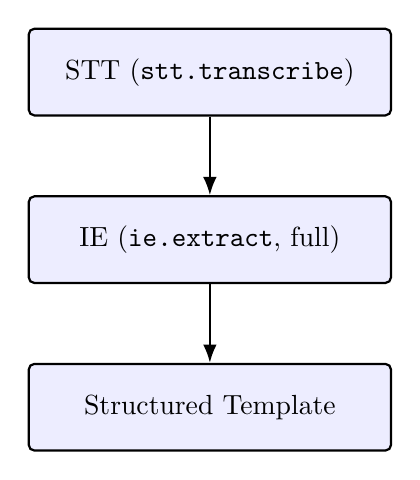
\begin{tikzpicture}[
  box/.style={draw, rounded corners=2pt, thick, minimum width=46mm,
              minimum height=11mm, align=center, fill=blue!7},
  arrow/.style={-Latex, thick}, node distance=10mm
]
\node[box] (stt) {STT (\texttt{stt.transcribe})};
\node[box, below=of stt] (ie) {IE (\texttt{ie.extract}, full)};
\node[box, below=of ie] (out) {Structured Template};

\draw[arrow] (stt) -- (ie);
\draw[arrow] (ie) -- (out);
\end{tikzpicture}%
}
\caption{S1 – Single-pass extraction.}
\end{figure}

\textbf{Notes.}  
\begin{itemize}
  \item Fastest: one LLM call after STT.  
  \item Fragile: any misclassification (e.g., “injured” vs “killed”) persists uncorrected.  
\end{itemize}

% ========================
\subsection*{Strategy S2: Per-Slot Extraction}

\textbf{Overview.}  
The orchestrator calls \texttt{ie.extract} once per slot (mode=\texttt{slot}), in parallel where possible. Each field is independently predicted.

\begin{figure}[H]
\centering
\resizebox{0.5\linewidth}{!}{%
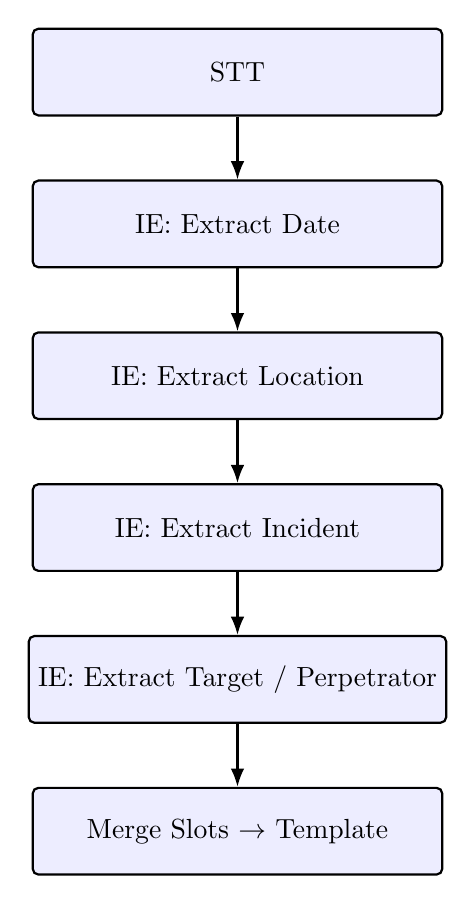
\begin{tikzpicture}[
  box/.style={draw, rounded corners=2pt, thick, minimum width=52mm,
              minimum height=11mm, align=center, fill=blue!7},
  arrow/.style={-Latex, thick}, node distance=8mm
]
\node[box] (stt) {STT};
\node[box, below=of stt] (q1) {IE: Extract Date};
\node[box, below=of q1] (q2) {IE: Extract Location};
\node[box, below=of q2] (q3) {IE: Extract Incident};
\node[box, below=of q3] (q4) {IE: Extract Target / Perpetrator};
\node[box, below=of q4] (merge) {Merge Slots $\rightarrow$ Template};

\draw[arrow] (stt) -- (q1);
\draw[arrow] (q1) -- (q2);
\draw[arrow] (q2) -- (q3);
\draw[arrow] (q3) -- (q4);
\draw[arrow] (q4) -- (merge);
\end{tikzpicture}%
}
\caption{S2 – Per-slot extraction.}
\end{figure}

\textbf{Notes.}  
\begin{itemize}
  \item Parallel execution reduces latency but increases cost (one call per slot).  
  \item Errors are isolated: a wrong date does not affect incident extraction.  
\end{itemize}

% ========================
\subsection*{Strategy S3: Single-Pass + Verification}

\textbf{Overview.}  
A full-template extraction (as in S1) is followed by \texttt{ver.verify}, which checks consistency, plausibility, and completeness. Low-confidence fields may trigger clarification.

\begin{figure}[H]
\centering
\resizebox{0.45\linewidth}{!}{%
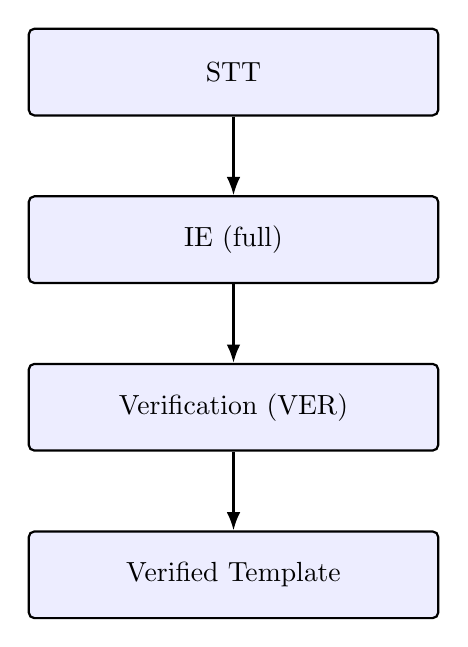
\begin{tikzpicture}[
  box/.style={draw, rounded corners=2pt, thick, minimum width=52mm,
              minimum height=11mm, align=center, fill=blue!7},
  arrow/.style={-Latex, thick}, node distance=10mm
]
\node[box] (stt) {STT};
\node[box, below=of stt] (ie) {IE (full)};
\node[box, below=of ie] (ver) {Verification (VER)};
\node[box, below=of ver] (out) {Verified Template};

\draw[arrow] (stt) -- (ie);
\draw[arrow] (ie) -- (ver);
\draw[arrow] (ver) -- (out);
\end{tikzpicture}%
}
\caption{S3 – Single-pass with verification.}
\end{figure}

\textbf{Notes.}  
\begin{itemize}
  \item Adds robustness by catching contradictions or implausible values.  
  \item If VER detects issues, orchestration can re-invoke IE with hints.  
\end{itemize}

% ========================
\subsection*{Strategy S4: Per-Slot + Verification}

\textbf{Overview.}  
Combines S2 (slot-wise extraction) with S3 (verification). Each slot is predicted independently and then verified.

\begin{figure}[H]
\centering
\resizebox{0.55\linewidth}{!}{%
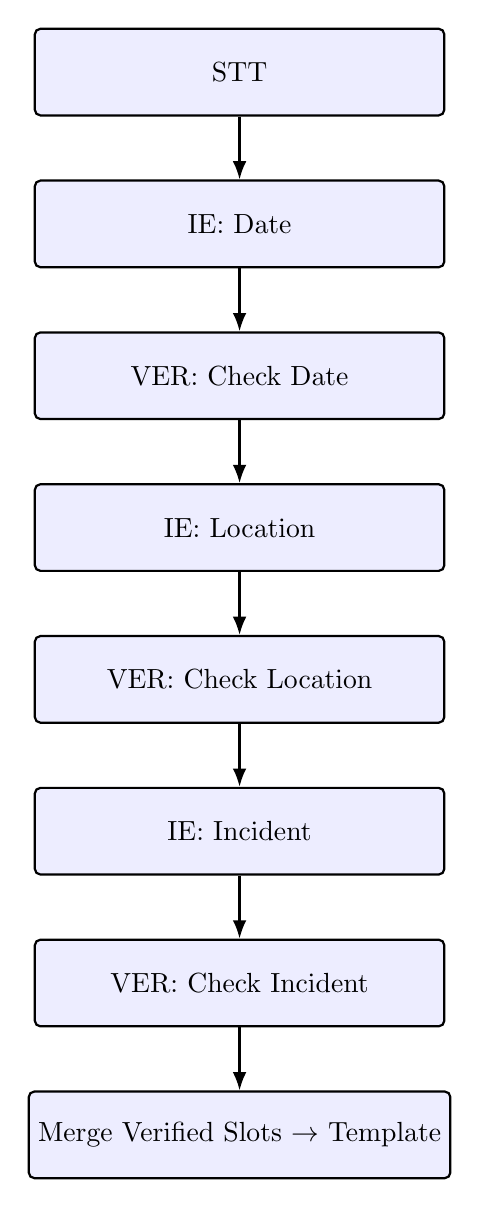
\begin{tikzpicture}[
  box/.style={draw, rounded corners=2pt, thick, minimum width=52mm,
              minimum height=11mm, align=center, fill=blue!7},
  arrow/.style={-Latex, thick}, node distance=8mm
]
\node[box] (stt) {STT};
\node[box, below=of stt] (q1) {IE: Date};
\node[box, below=of q1] (v1) {VER: Check Date};
\node[box, below=of v1] (q2) {IE: Location};
\node[box, below=of q2] (v2) {VER: Check Location};
\node[box, below=of v2] (q3) {IE: Incident};
\node[box, below=of q3] (v3) {VER: Check Incident};
\node[box, below=of v3] (merge) {Merge Verified Slots $\rightarrow$ Template};

\draw[arrow] (stt) -- (q1);
\draw[arrow] (q1) -- (v1);
\draw[arrow] (v1) -- (q2);
\draw[arrow] (q2) -- (v2);
\draw[arrow] (v2) -- (q3);
\draw[arrow] (q3) -- (v3);
\draw[arrow] (v3) -- (merge);
\end{tikzpicture}%
}
\caption{S4 – Per-slot extraction with verification.}
\end{figure}

\textbf{Notes.}  
\begin{itemize}
  \item Highest reliability: each slot is validated independently.  
  \item Computationally most expensive. Best suited for high-stakes use cases.  
\end{itemize}

% ========================
\subsection*{Summary}

The orchestrator can switch between strategies without altering agent implementations, as all share the same JSON contracts. This separation allows empirical evaluation of trade-offs between cost, accuracy, and robustness in later chapters.

\section{User Interface}
\label{sec:user-interface}

The user interface implements the human-in-the-loop quality control paradigm established in Section~\ref{sec:system-workflow}. The interface design focuses on efficient template filling through voice input and interactive correction workflows.

\subsection{Authentication and Template Access}
\label{subsec:ui-authentication}

The system implements role-based access through a centralized authentication interface (Figure~\ref{fig:login-interface}). Users authenticate via Keycloak-managed credentials, which determine which template types they can access. Security personnel see incident reporting templates, while medical staff access patient handover forms. Users cannot create new template schemas through the interface—they can only fill templates assigned to their role.

\begin{figure}[H]
  \centering
  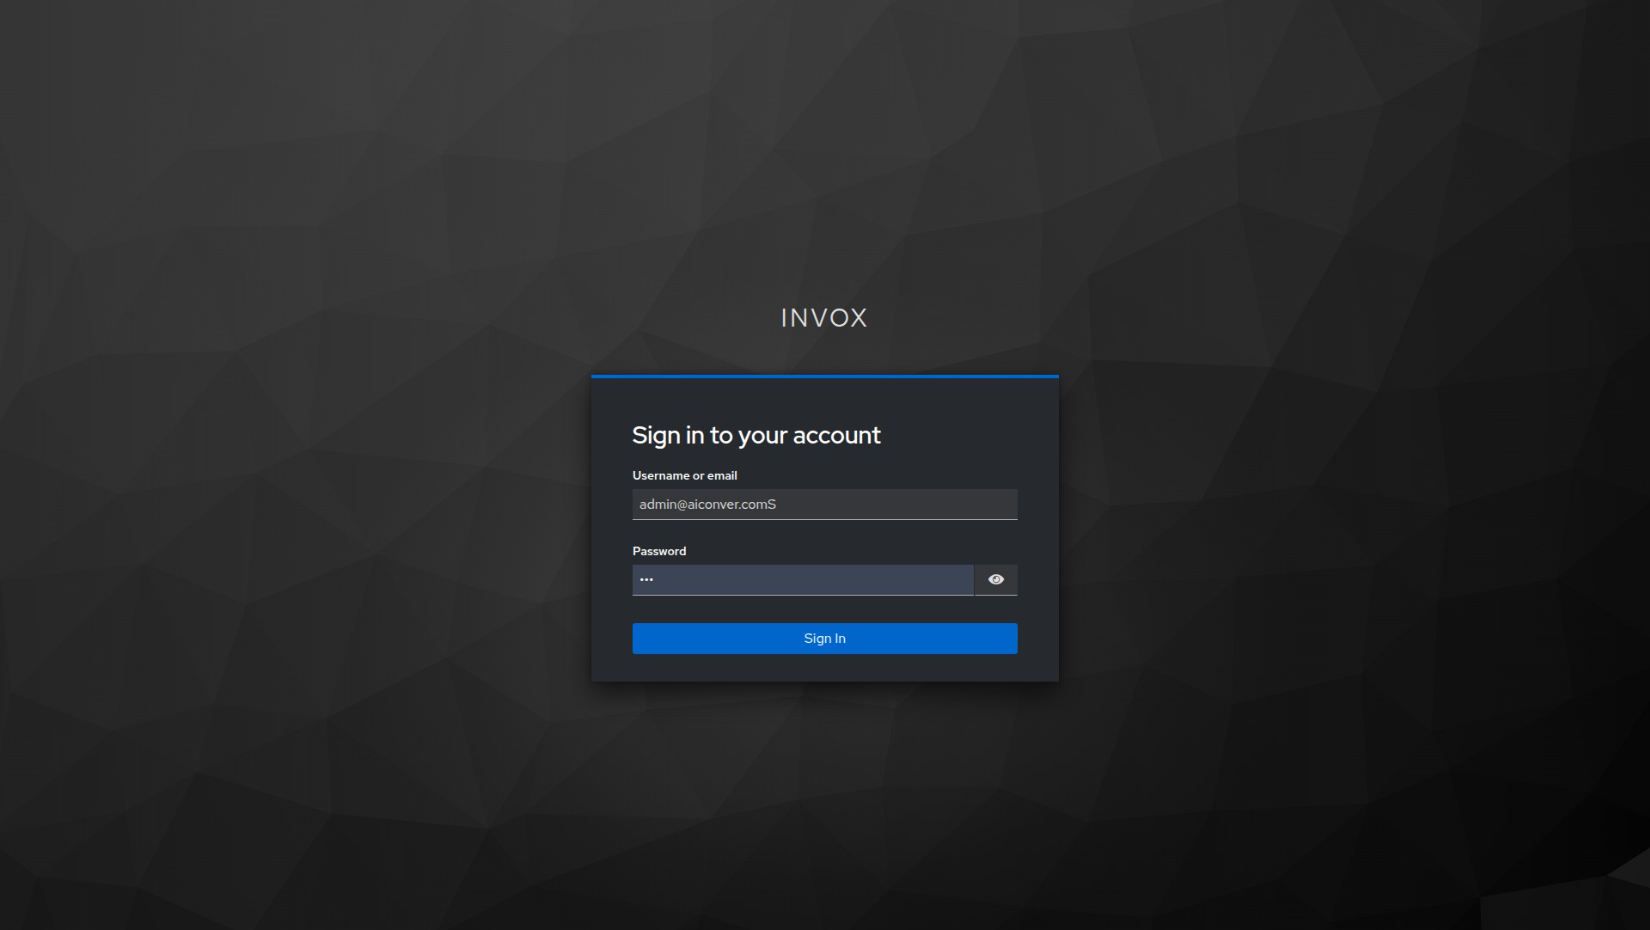
\includegraphics[width=1.0\linewidth]{images/login_interface.png}
  \caption{INVOX authentication interface with Keycloak integration}
  \label{fig:login-interface}
\end{figure}

\subsection{Template Filling Interface}
\label{subsec:ui-template-filling}

\begin{figure}[H]
  \centering
  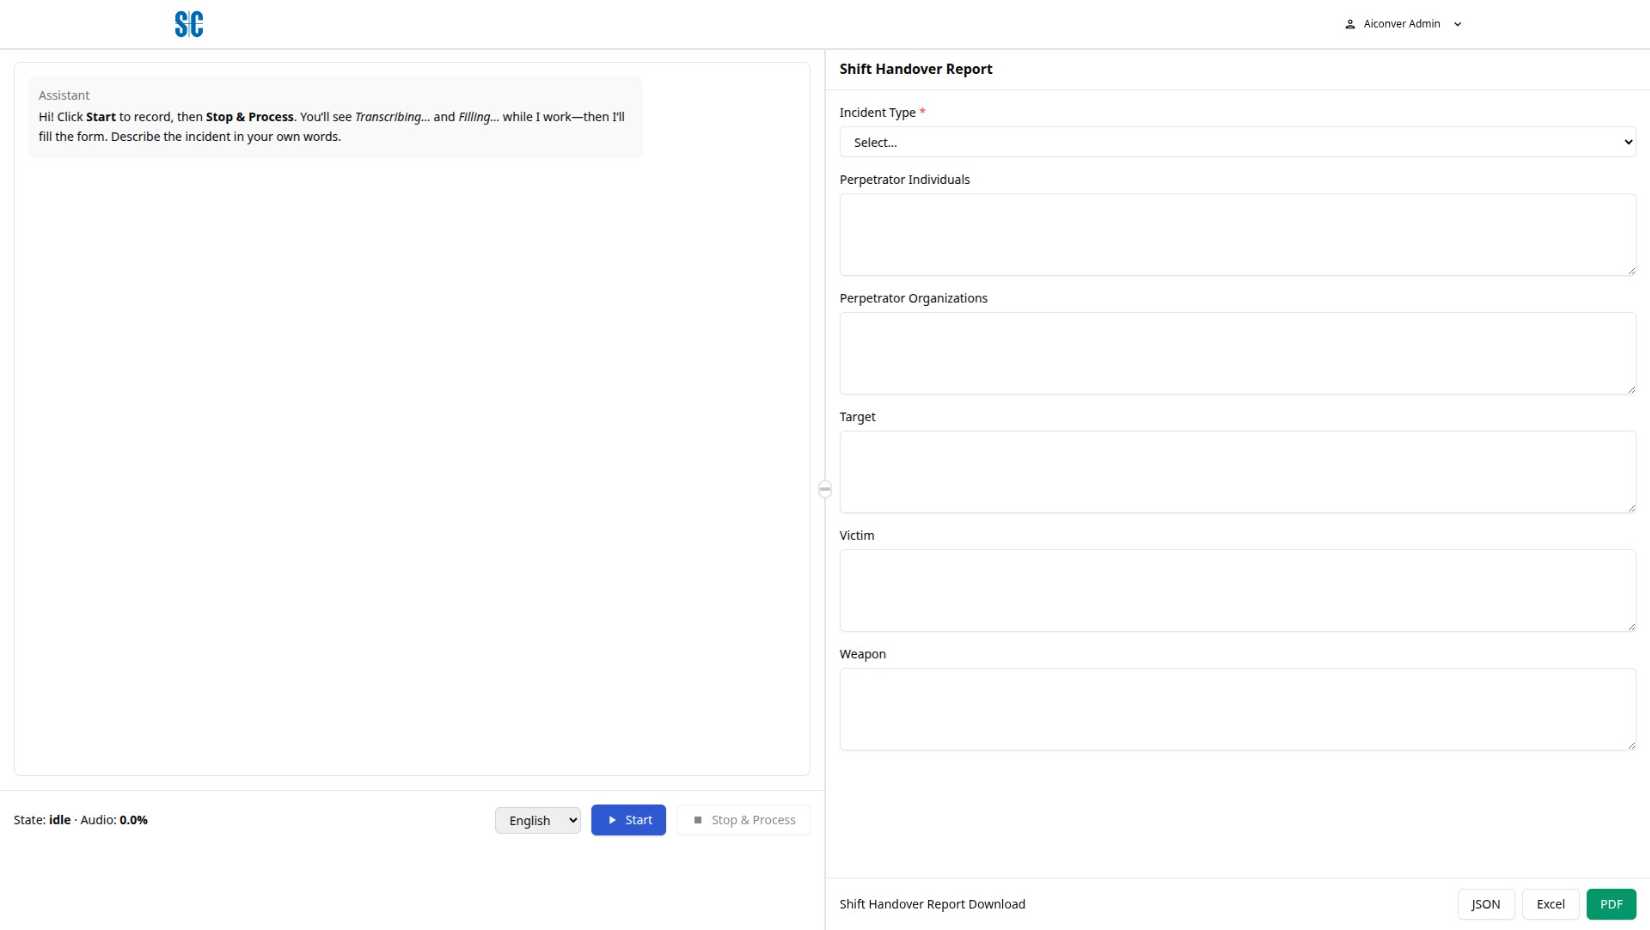
\includegraphics[width=1.0\linewidth]{images/template_interface.png}
  \caption{Template filling interface with voice input (bottom-left), structured form (right), and interactive chat panel}
  \label{fig:template-interface}
\end{figure}

The interface consists of three main components (Figure~\ref{fig:template-interface}): the audio recording panel at the bottom-left, the structured template form on the right, and an interactive chat panel for clarifications.

\subsubsection{Audio Recording Panel}

The recording panel provides a "Start" button to initiate audio capture. During recording, the button changes to "Stop \& Process." When clicked, the system transcribes the audio and extracts template values using the selected strategy. A strategy selector menu allows users to choose between S1, S2, S3, or S4 before processing, enabling them to balance speed versus accuracy based on the template's importance.

\subsubsection{Structured Template Form}

The right side displays the template form with fields organized by category (Incident Type, Perpetrator Information, Target, Victim, Weapon). As the system processes audio input, fields are automatically populated based on the extraction results. Each field type renders appropriately: dropdowns for enumerated values, text areas for descriptions, and specialized inputs for dates and numbers. Fields populated by AI extraction are marked with confidence indicators, with low-confidence fields highlighted to direct user attention.

Users can directly edit any field value, lock fields to prevent overwriting during subsequent recordings, and review the source of each value (AI-extracted versus manually entered). The form validates inputs against schema constraints before allowing submission.

\subsubsection{Interactive Chat Panel}

The chat panel provides real-time feedback during template filling. When the system identifies missing required fields, conflicting information, or ambiguous extractions, it posts messages requesting clarification. For example, if the perpetrator field contains uncertain information, the chat prompts the user to provide more specific details. This interactive guidance reduces iteration cycles by identifying issues immediately rather than after submission.

\subsection{Template Export}

Once users complete template review, the interface provides export options in JSON, Excel, and PDF formats through a download button group. All templates are automatically persisted to PostgreSQL upon processing, ensuring data preservation regardless of export actions.

Having established the complete implementation of the Invox system—from backend agent architecture to frontend user interface—the next chapter evaluates this implementation empirically. Chapter~\ref{chap:evaluation} applies the system to the MUC-4 benchmark and measures its performance against the six requirements (R1–R6) established in Chapter~\ref{chap:requirements}. The evaluation compares the four architectural strategies quantitatively, examining their trade-offs in accuracy, cost, latency, and user satisfaction.

% Add more chapters as needed...
% \chapter{Concept}
% \chapter{Implementation}
% ...

% =====================================================
% BACKMATTER: Bibliography, Index, etc.
% =====================================================
\backmatter

\bibliographystyle{splncs03}
\bibliography{bibliography}

\printindex

\end{document}
